% !TEX root = handbook-physics.tex
% !TEX TS-program = pdflatex
% !TEX encoding = UTF-8 Unicode




\chapter[Structure Of Atoms And Molecules]{Structure Of Atoms And Molecules And Their Optical Properties}
\label{ch-39}
\zhtitle{原子和分子的结构及其光学性质}

\section{The Hydrogen Atom and Hydrogen-Like Ions}
\label{sec-39.1} 
\zhtitle{氢原子与类氢离子}

\subsection{}\label{39.1.1} An \redem{atom} is the smallest particle of matter possessing all the chemical properties of the given chemical element. An atom consists of a positively charged nucleus and electrons moving about in the electric field of the nucleus. The nuclear charge $Ze$ \ssect{42.1.2} is equal in magnitude to the total charge of all the electrons
of the atom. An ion is the electrically charged particle formed when an atom or molecule loses or gains electrons.
\zhpar{原子是保持给定化学元素全部化学性质的最小粒子。原子由带正电的原子核和在原子核电场中运动的电子组成。原子核的电荷 $Ze$ \ssect{42.1.2} 在数值上等于原子中全部电子的总电荷。离子是原子或分子失去或获得电子后形成的带电粒子。}

\subsection{}\label{39.1.2} The simplest atomic system is the hydrogen atom, consisting of a single proton in the nucleus and a single electron moving in the Coulomb field of the nucleus. \redem{Hydrogen-like ions (isoelectronic with hydrogen)} are such as \ce{He+}, \ce{Li^{3+}}, and \ce{Be^{2+}}, which also have a nucleus with the charge Ze and a single electron.
\zhpar{最简单的原子体系是氢原子，它由原子核中的一个质子和在原子核库仑场中运动的一个电子组成。\redem{类氢离子（与氢等电子）}如 \ce{He+}、\ce{Li^{3+}} 和 \ce{Be^{2+}} 等，它们的原子核同样带有电荷 $Ze$，并且同样只有一个电子。}

\subsection{}\label{39.1.3} Among the optical properties of atoms, the most important is their emission spectrum. The frequency $\nu$ of the lines in the discrete line spectrum of hydrogen is described by the Balmer-Rydberg formula:
\zhpar{在原子的光学性质中，最重要的是其发射光谱。氢的线状光谱中谱线的频率 $\nu$ 由巴耳末-里德伯公式描述：}
\begin{equation*}%
\nu = cR' \left( \frac{1}{n^{2}} - \frac{1}{m^{2}} \right) = R \left( \frac{1}{n^{2}} - \frac{1}{m^{2}} \right),
\end{equation*}
where
\zhpar{式中：}
\begin{align*}%
R & = \frac{me^{4}}{8 \varepsilon_{0}^{2} h^{3}} \text{ in SI units},\\
R & = \frac{2 \pi^{2} me^{4}}{h^{3}} \text{(in Gaussian units).}
\end{align*}
Here $c$ is the velocity of light in free space, $m$ is the mass of the electron, $e$ is the electron charge, $h$ is Planck's constant, and $\varepsilon_{0}$ is the electric constant in SI units \ssect{14.2.7}.
\zhpar{式中 $c$ 为真空中的光速，$m$ 为电子质量，$e$ 为电子电荷，$h$ 为普朗克常量，$\varepsilon_{0}$ 为 SI 单位制中的真空电容率 \ssect{14.2.7}。}

Quantities $R$ and $R' = R/c$ are called the \redem{Rydberg constant} in \si{\per\second} and in \si{\per\centi\meter} or \si{\per\meter}, respectively: $R = \SI{3.2931193d15}{\per\second}$ and $R' = \SI{1.0973731d7}{\per\meter}$.
\zhpar{量 $R$ 和 $R' = R/c$ 分别称为\redem{里德伯常量}，它们的单位分别为 \si{\per\second} 和 \si{\per\centi\meter}（或 \si{\per\meter}）。其数值为：$R = \SI{3.2931193d15}{\per\second}$，$R' = \SI{1.0973731d7}{\per\meter}$。}

The whole numbers $n$ and $m$ are called the \redem{principal quantum numbers}, and $m = n + 1$, $n + 2$, etc. A group of lines having the same $n$ value is called a \redem{series}. The hydrogen spectrum has the following series: \redem{Lyman series} at $n = 1$, \redem{Balmer series} at $n = 2$, \redem{Paschen series} at $n = 3$, \redem{Brackett series} for $n = 4$, \redem{Pfund series} for $n = 5$ and the \redem{Humphreys series} for $n = 6$.
\zhpar{整数 $n$ 和 $m$ 称为\redem{主量子数}，且 $m = n + 1$、$n + 2$ 等等。具有相同 $n$ 值的一组谱线称为一个\redem{谱线系}。氢原子光谱包含下列谱线系：$n = 1$ 对应\redem{莱曼系}，$n = 2$ 对应\redem{巴耳末系}，$n = 3$ 对应\redem{帕邢系}，$n = 4$ 对应\redem{布拉开系}，$n = 5$ 对应\redem{普丰德系}，$n = 6$ 对应\redem{汉弗莱系}。}

For hydrogen-like ions \ssect{39.1.1} the Balmer-Rydberg formula is
\zhpar{对于类氢离子 \ssect{39.1.1}，巴耳末-里德伯公式为：}
\begin{equation*}%
\nu = Z^{2}R \left( \frac{1}{n^{2}} - \frac{1}{m^{2}} \right),
\end{equation*}
where $Z$ is the atomic number of the element in the Mendeleev periodic table \ssect{39.3.5}.
\zhpar{式中 $Z$ 为元素在门捷列夫周期表中的原子序数 \ssect{39.3.5}。}


\subsection{}\label{39.1.4} Each value of the quantum number $n$ in the Balmer-Rydberg formula corresponds to the series limit with the maximum frequency (at $m = \infty$), called the \redem{term} $T_{n}$. Thus
\zhpar{巴耳末-里德伯公式中量子数 $n$ 的每一个取值，都对应于频率最大的谱线系限（$m = \infty$）。该系限所对应的量称为\redem{光谱项} $T_{n}$。于是有：}
\begin{align*}%
T_{n} & = \frac{R}{n^{2}} \text{ (for hydrogen),}\\
T_{n} & = \frac{Z^{2}R}{n^{2}} \text{ (for hydrogen-like ions).}
\end{align*}

\subsection{}\label{39.1.5} The energy of a hydrogen-like ion in a state with the principal quantum number $n$ is:
\zhpar{处于主量子数为 $n$ 的状态时，类氢离子的能量为：}
\begin{equation*}%
E_{n} = - \frac{Z^{2}Rh}{n^{2}}, \quad T_{n} = \frac{\abs{E_{n}}}{h}.
\end{equation*}
The magnitude $E_{n}$ is called the \redem{binding energy} of the electron in the atom. The minimum value $E_{1}$ (at $n = 1$) corresponds to the ground, or normal, state of the atom \ssect{39.1.9}. All energy values at $n > 1$ characterize \redem{excited states of the atom}. The most vital distinguishing feature of excited states is the finite lifetime t of the electron in these states: $\tau \approx \SI{d-8}{\second}$. In the ground state of the atom, isolated from all external effects, $\tau$ is unlimited.
\zhpar{$E_{n}$ 的绝对值称为电子在原子中的\redem{结合能}。最小值 $E_{1}$（$n = 1$）对应于原子的基态，即正常态 \ssect{39.1.9}。所有 $n > 1$ 的能量值都描述原子的\redem{激发态}。激发态最主要的区别特征是电子在这些状态中的寿命 $\tau$ 有限，$\tau \approx \SI{d-8}{\second}$。原子处于基态且与一切外界作用隔绝时，$\tau$ 是无限的。}

The maximum energy value  $E_{\mathrm{max}} = 0$ as $n \to \infty$ corresponds to \redem{ionization} of the atom or \redem{ion}, i.e. to the removal of an electron from it.
\zhpar{当 $n \to \infty$ 时 $E_{\mathrm{max}} = 0$，这对应于原子或离子的\redem{电离}，即从原子中移去一个电子。}

In magnitude, the ionization energy is equal to the binding
energy of an electron in the atom (or ion).
\zhpar{在数值上，电离能等于原子（或离子）中电子的结合能。}

The \redem{ionization potential} \ssect{16.2.6} of an atom of hydrogen or of a hydrogen-like ion in the state with the principal quantum number $n$ is equal to $V = Z^{2}Rh/en^{2}$, where $e$ is the magnitude of the charge of the electron. A diagram of the energy levels in the hydrogen atom and the arrangement of its series of spectral lines are given in \figr{fig-39-01}. 
\zhpar{氢原子或类氢离子在主量子数为 $n$ 的状态下的\redem{电离电势} \ssect{16.2.6} 为 $V = Z^{2}Rh/en^{2}$，式中 $e$ 为电子电荷的大小。氢原子的能级图及其谱线系的排列见\figr{fig-39-01}。}

\begin{figure}%[-3cm]
\centering
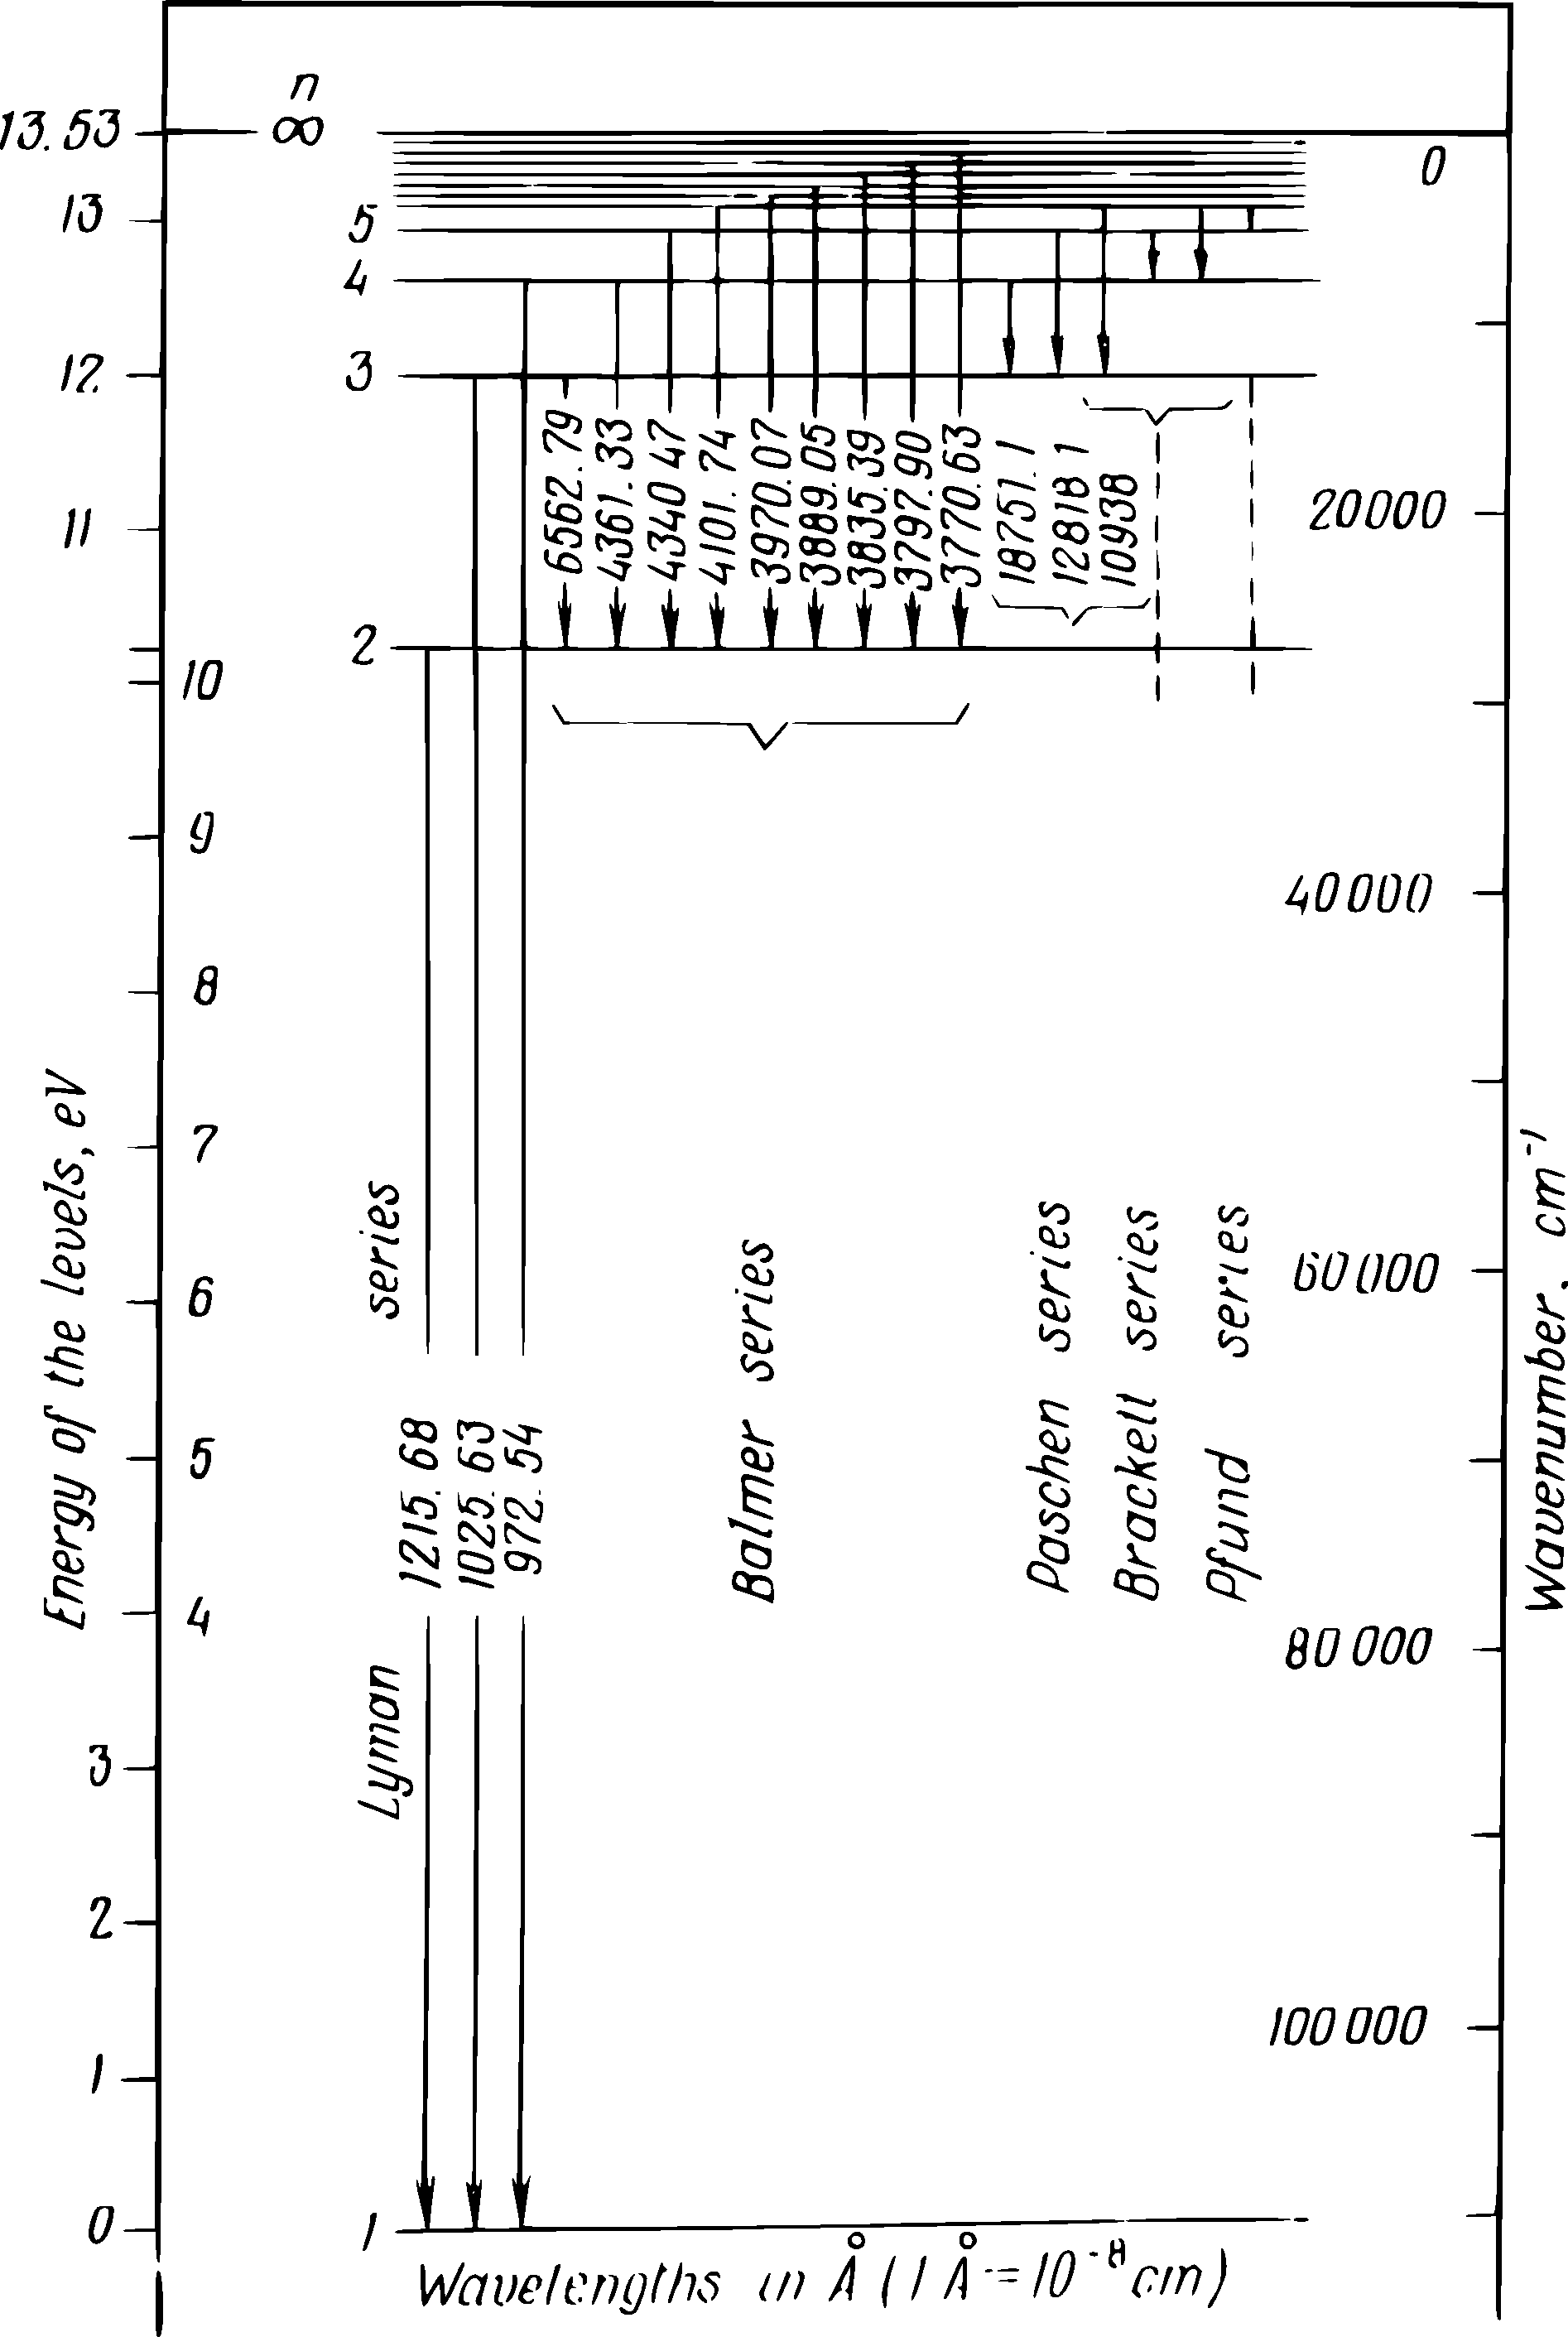
\includegraphics[height=0.9\textheight]{figs/ch-39/fig-39-01.pdf}
\sidecaption[][-5cm]{A diagram of the energy levels in the hydrogen atom and the arrangement of its series of spectral lines.\zhcap{氢原子能级图及其谱线系的排列。}\label{fig-39-01}}
\end{figure}


\subsection{}\label{39.1.6} The spectrum and the energy levels of the hydrogen atom were first interpreted by means of Bohr's postulates. \redem{Bohr's first postulate (steady states postulate)} states that there are a set of stationary, or steady, states of the atom in which it does not radiate electromagnetic waves. The steady states correspond to steady orbits \ssect{39.1.8} along which electrons travel with acceleration, but no light is radiated (cf. \ssect{31.3.4}).
Bohr's first postulate was explained by quantum mechanics
\ssect{38.2.6}.
\zhpar{氢原子的光谱和能级最初是借助玻尔公设来解释的。\redem{玻尔第一公设}（定态公设）指出：原子存在一系列稳定的定态，在这些状态中原子不辐射电磁波。定态对应于定态轨道 \ssect{39.1.8}，电子沿这些轨道运动时具有加速度，但不辐射光（参见 \ssect{31.3.4}）。玻尔第一公设已由量子力学 \ssect{38.2.6} 加以解释。}

\redem{Bohr's second postulate (orbit quantization rule)} states that in the steady state of the atom, the electron, travelling along a circular orbit, has quantized values of its angular momentum that comply with the condition
\zhpar{\redem{玻尔第二公设}（轨道量子化条件）指出：原子处于定态时，沿圆轨道运动的电子，其角动量取量子化的值，满足下列条件：}
\begin{equation*}%
L_{k} = mvr = k \hbar \quad (k = 1,\, 2,\, 3,\,\ldots{}).
\end{equation*}
Mere $m$ is the mass of the electron, $v$ is its velocity, $r$ is the radius of the $k$th orbit, and $\hbar = h/2\pi$. The whole number $k$ is equal to the number of de Broglie wavelengths for the electron \ssect{38.1.4} per length of the circular orbit: 
\zhpar{式中 $m$ 为电子质量，$v$ 为其速度，$r$ 为第 $k$ 个轨道的半径，$\hbar = h/2\pi$。整数 $k$ 等于圆轨道周长中所容纳的电子德布罗意波长的个数，即：}
\begin{equation*}%
\frac{2\pi r}{\lambda} = \frac{2 \pi r mv}{h} = k.
\end{equation*}
The quantization of the angular momentum in quantum mechanics
is discussed in \ssect{39.1.8}.
\zhpar{在量子力学中，角动量的量子化问题见 \ssect{39.1.8}。}

\redem{Bohrs third postulate (the Bohr frequency condition)} states that in going from one steady state orbit to another, the atom either emits or absorbs one photon. A photon is emitted when the atom passes from a state with more energy to one with less energy. Upon transition in the opposite direction, a photon is absorbed. The energy $h \nu$ of the photon is equal to the difference in energy in the two states. Thus
\zhpar{\redem{玻尔第三公设}（玻尔频率条件）指出：原子从一个定态轨道跃迁到另一个定态轨道时，要么发射一个光子，要么吸收一个光子。原子由能量较高的状态跃迁到能量较低的状态时发射光子；反向跃迁时则吸收光子。光子的能量 $h \nu$ 等于两状态的能量差。于是有：}
\begin{equation*}%
E_{n} - E_{m} = h\nu.
\end{equation*}
When $E_{n} > E_{m}$ a photon is emitted; when $E_{n} < E_{m}$ a photon is absorbed.
\zhpar{当 $E_{n} > E_{m}$ 时发射光子；当 $E_{n} < E_{m}$ 时吸收光子。}

In quantum mechanics, Bohr's frequency condition follows from
the theory of quantum transitions from one energy state to
another. Information on this theory is beyond the scope of the
present handbook.
\zhpar{在量子力学中，玻尔频率条件可由能量状态之间量子跃迁的理论导出。有关该理论的内容超出了本手册的范围。}

\subsection{}\label{39.1.7} Schr\"odinger's steady-state equation \ssect{38.2.5} for the motion of an electron in the Coulomb field of a nucleus with the charge $Ze$ \ssect{42.1.2} is of the form 
\zhpar{电子在电荷为 $Ze$ \ssect{42.1.2} 的原子核库仑场中运动时，其定态薛定谔方程 \ssect{38.2.5} 的形式为：}
\begin{equation*}%
\laplacian \psi + \frac{2m}{\hbar^{2}} (E - U) \psi = 0,
\end{equation*}
where $U (r) = -Ze^{2}/4\pi \varepsilon_{0} r$ is the potential energy of an electron located at the distance $r$ from the nucleus, $\varepsilon_{0}$ is the electric constant in SI units \ssect{14.2.7}, and $E$ is the total energy of the electron in the atom, which it is necessary to determine under the assumption that the wave functions $\psi$ comply with the conditions indicated in \ssect{38.2.4}.
\zhpar{式中 $U (r) = -Ze^{2}/4\pi \varepsilon_{0} r$ 为距原子核为 $r$ 处电子的势能，$\varepsilon_{0}$ 为 SI 单位制中的真空电容率 \ssect{14.2.7}，$E$ 为原子中电子的总能量。$E$ 需要在假定波函数 $\psi$ 满足 \ssect{38.2.4} 中所给条件的前提下求出。}

\subsection{}\label{39.1.8} A solution of the Schr\"odinger steady-state equation for an electron in a centrally symmetrical Coulomb field of the nucleus yields the following:
\zhpar{求解电子在中心对称库仑场中的定态薛定谔方程，可得到下列结果：}
\begin{enumerate}[label=(\alph*)]
\item the angular momentum of the electron in the atom is quantized according to the formula:
\zhpar{原子中电子的角动量按下式量子化：}
\begin{equation*}%
L_{l} = \sqrt{l(l + 1)} \, \hbar,
\end{equation*}
where the \redem{orbital quantum number} $l$, determining the angular momentum, varies within the limits: $l = 0,\,\ 1,\, \ldots{}, (n - 1)$, where $n$ is the principal quantum number \ssect{39.1.3};
\zhpar{式中，决定角动量的\redem{轨道量子数} $l$ 的取值范围为 $l = 0,\ 1,\ \ldots, (n - 1)$，其中 $n$ 为主量子数 \ssect{39.1.3}；}
\item at $E < 0$, when the electron is ``bound'' in the atom, its motion is periodic, and the value of the total energy $E$ is quantized. The eigenvalues $E_{n}$ \ssect{38.2.5} are determined by the formula:
\zhpar{当 $E < 0$ 时，电子被“束缚”在原子中，其运动是周期性的，总能量 $E$ 取量子化的值。能量本征值 $E_{n}$ \ssect{38.2.5} 由下式确定：}
\begin{align*}%
E_{n} & = - \frac{Z^{2}me^{4}}{8 h^{2} \varepsilon_{0}^{2}} & = - \frac{Z^{2}R h }{n^{2}} && \text{(in SI units)},\\
E_{n} & = - \frac{2 \pi^{2} Z^{2}me^{4}}{h^{2}} & = - \frac{Z^{2}R h }{n^{2}} && \text{(in Gaussian units).}
\end{align*}
Here $R$ is the Rydberg constant \ssect{39.1.3}. The solution of the Schr\"odinger equation for an electron in a hydrogen-like ion leads to energy levels of the Balmer-Rydberg type \ssect{39.1.4}.
\zhpar{式中 $R$ 为里德伯常量 \ssect{39.1.3}。求解类氢离子中电子的薛定谔方程，得到的能级具有巴耳末-里德伯型 \ssect{39.1.4}。}
\end{enumerate}
\subsection{}\label{39.1.9} In accordance with the orbital quantum number, the following letters have been assigned to designate the state of the electron in atoms:\\
$s$-state at $l = 0$, $p$-state at $l = 1$,\\
$d$-state at $l = 2$, $f$-state at $l = 3$, etc.
\zhpar{根据轨道量子数，人们用下列字母表示原子中电子的状态：$l = 0$ 时为 $s$ 态，$l = 1$ 时为 $p$ 态，$l = 2$ 时为 $d$ 态，$l = 3$ 时为 $f$ 态，依此类推。}

The $s$-state of the electron in the hydrogen atom at $n = 1$ is called the ground state (see also \ssect{39.1.5}). This state is spherically symmetrical. The wave function of this state depends only upon the distance $r$ of the electron from the nucleus $[\psi = \psi (r)]$ and is of the form
\zhpar{氢原子中 $n = 1$ 时电子的 $s$ 态称为基态（另见 \ssect{39.1.5}）。该态具有球对称性。此态的波函数仅依赖于电子到原子核的距离 $r$，即 $[\psi = \psi (r)]$，其形式为：}
\begin{equation*}%
\psi = \psi(r) = C \exp \left( -\frac{r}{a_{0}} \right),
\end{equation*}
where $C$ is a constant determined from the normalization condition for probabilities \ssect{38.2.2}, and $a_{0}$ is the first Bohr radius:
\zhpar{式中 $C$ 为由概率归一化条件 \ssect{38.2.2} 确定的常量，$a_{0}$ 为第一玻尔半径：}
\begin{align*}%
a_{0} & = \frac{4 \pi \varepsilon_{0} \hbar^{2}}{m e^{2}} && \text{(in SI units)},\\
E_{n} & = \frac{\hbar^{2}}{m e^{2}} && \text{(in Gaussian units).}
\end{align*}
In quantum mechanics, the electron orbits in the atom are considered to be the locus of points at which the probability of finding the electron is a maximum. In particular, for the $s$-state of the hydrogen atom, such an orbit is the first circular Bohr orbit of a radius equal to $a_{0}$.
\zhpar{在量子力学中，原子中电子的轨道被看作电子出现概率最大的点的轨迹。特别地，对于氢原子的 $s$ 态，这种轨道就是半径等于 $a_{0}$ 的第一个圆形玻尔轨道。}

\section{Space Quantization}
\label{sec-39.2} 

\begin{marginfigure}%[-3cm] 
\centering
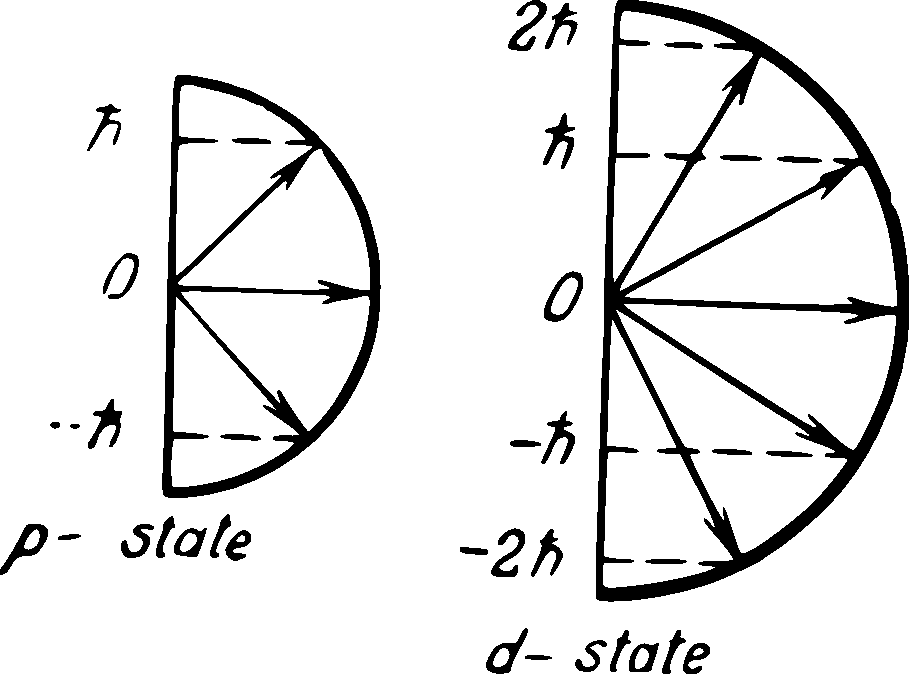
\includegraphics[width=\textwidth]{figs/ch-39/fig-39-02.pdf}
\sidecaption{The space quantization of vectors $\vb{L}_{l}$ for electrons in $p$- and $d$-states.\zhcap{电子处于 $p$ 态和 $d$ 态时矢量 $\vb{L}_{l}$ 的空间量子化。}\label{fig-39-02}}
\end{marginfigure}

\subsection{}\label{39.2.1} \redem{Space quantization} is the existence of definite discrete orientations in space of the angular momentum vector $\vb{L}_{l}$ of the electron. This phenomenon has been proven in quantum mechanics. The only allowed orientations of $\vb{L}_{l}$ are those in which
the projection ${L}_{lz}$ of vector $\vb{L}_{l}$ along the direction $Z$ of the external magnetic, field assumes values that are multiples of $\hbar$.
Thus
\zhpar{空间量子化是指电子角动量矢量 $\vb{L}_{l}$ 在空间中具有确定的离散取向。这一现象已在量子力学中得到证明。$\vb{L}_{l}$ 唯一允许的取向，是使其在外磁场方向 $Z$ 上的投影 ${L}_{lz}$ 取 $\hbar$ 的整数倍的那些取向。于是有：}
\begin{equation*}%
L_{lz}= m \hbar,
\end{equation*}
where $m$ is a whole number called the \redem{magnetic quantum number} and assumes the values $m = 0, \, \pm 1, \, \pm 2, \ldots{},$ and $l$ is the orbital quantum number \ssect{39.1.8}. Given in \figr{fig-39-02} is the space quantization of vectors $L_{l}$ for electrons in the $p$- and $d$-states \ssect{39.1.9}.
\zhpar{式中 $m$ 为称为\redem{磁量子数}的整数，它取值为 $m = 0, \, \pm 1, \, \pm 2, \ldots{}$，$l$ 为轨道量子数 \ssect{39.1.8}。\figr{fig-39-02}给出了电子处于 $p$ 态和 $d$ 态时矢量 $L_{l}$ 的空间量子化情况 \ssect{39.1.9}。}


\subsection{}\label{39.2.2} Since the angular momentum vector of the electron is proportional to the orbital magnetic moment of the electron \ssect{26.1.2}, it follows from space quantization that the vector $\vb{p}_{m}$ of the orbital magnetic moment of the electron \ssect{26.1.2} in the external magnetic field cannot assume arbitrary orientations.
\zhpar{由于电子的角动量矢量与电子的轨道磁矩成正比 \ssect{26.1.2}，由空间量子化可知，外磁场中电子的轨道磁矩矢量 $\vb{p}_{m}$ 不能取任意取向。}

\subsection{}\label{39.2.3} It was experimentally established that space quantization is observed in atoms having a single outer-shell (valence) electron in the $s$-state (where $l = 0$) \ssect{39.1.9}. In this state the atoms lack angular momentum ($L_{0} = 0$; see \ssect{39.1.8}. Space quantization,
detected in such experiments, pertained to electron spin, and confirmed the existence of two possible spin orientations in the external magnetic field \ssect{26.1.3}.
\zhpar{实验证实，只有在外层（价）电子处于 $s$ 态（$l = 0$）的原子中才能观察到空间量子化 \ssect{39.1.9}。在这种状态下，原子没有角动量（$L_{0} = 0$；见 \ssect{39.1.8}）。这类实验中探测到的空间量子化与电子自旋有关，证实了外磁场中电子自旋有两种可能的取向 \ssect{26.1.3}。}

The magnitude of the spin angular momentum $L_{ls}$ of the electron is determined by the formula \ssect{39.1.8}:
\zhpar{电子自旋角动量 $L_{ls}$ 的大小由下式确定 \ssect{39.1.8}：}
\begin{equation*}%
L_{ls}= \sqrt{s\, (s+1)}\, \hbar,
\end{equation*}
where $s$ is the \redem{spin quantum number}, equal to $s = 1/2$. Therefore, the numerical value of electron spin equals \ssect{26.1.3}:
\zhpar{式中 $s$ 为\redem{自旋量子数}，$s = 1/2$。因此，电子自旋的数值为 \ssect{26.1.3}：}
\begin{equation*}%
L_{ls}= \sqrt{\frac{1}{2} \left( \frac{1}{2} + 1 \right)} \, \hbar = \frac{\sqrt{3}}{2} \,\hbar,
\end{equation*}
Space quantization of spin means that the projection $L_{lsz}$
of the spin vector $\vb{L}_{ls}$ on the direction of the external magnetic field is determined by the formula
\zhpar{自旋的空间量子化意味着，自旋矢量 $\vb{L}_{ls}$ 在外磁场方向上的投影 $L_{lsz}$ 由下式确定：}
\begin{equation*}%
L_{lsz}= m_{s} \, \hbar,
\end{equation*}
where $m_{s}$ is the \redem{spin magnetic quantum number}, differing from the spin quantum number s in that it can assume two values: not only $+1/2$, but $-1/2$ as well.\sidenote{Frequently, no distinction is made between the two spin quantum numbers $s$ and $m_{s}$, referring, in this case, to $m_{s}$ to which two values, $\pm 1/2$, are assigned.}
\zhpar{式中 $m_{s}$ 为\redem{自旋磁量子数}，它与自旋量子数 $s$ 的不同之处在于，它可取两个值：不仅可取 $+1/2$，还可取 $-1/2$。}
\zhpar{注：通常不区分两个自旋量子数 $s$ 和 $m_{s}$，此时所说的 $m_{s}$ 即指取 $\pm 1/2$ 两个值的量。}

\section[Pauli Exclusion Principle. Periodic Table]{Pauli Exclusion Principle. Mendeleev's Periodic Table}
\label{sec-39.3} 
\zhtitle{泡利不相容原理。门捷列夫元素周期表}




\subsection{}\label{39.3.1} The simplest statement of the \redem{Pauli exclusion principle}is: in any atom there cannot be two electrons occupying two identical steady states, which are specified by a set of four quantum numbers: the principal $n$ , orbital $l$, magnetic $m$ and spin magnetic $m_{s}$ quantum numbers.
\zhpar{\redem{泡利不相容原理}最简单的表述是：在任何原子中，不可能有两个电子占据完全相同的定态。这些定态由一组四个量子数确定，即主量子数 $n$、轨道量子数 $l$、磁量子数 $m$ 和自旋磁量子数 $m_{s}$。}

Also obeying the Pauli principle, in addition to electrons, are other particles having half-integral spin (in $\hbar$ units). In any system of fermions \ssect{41.2.4} no two particles can exist in identical quantum states \ssect{41.1.4}.
\zhpar{除电子外，自旋为半整数（以 $\hbar$ 为单位）的其他粒子也服从泡利原理。在任何费米子体系 \ssect{41.2.4} 中，不可能有两个粒子处于相同的量子态 \ssect{41.1.4}。}

For the electrons in an atom, the Pauli principle is written as follows:
\zhpar{对于原子中的电子，泡利原理可写成下列形式：}
\begin{equation*}%
Z_{1} (n,\, l, \, m,\, m_{s}) = 0 \text{ or } 1,
\end{equation*}
where $Z_{1} (n,\, l, \, m,\, m_{s})$ is the number of electrons in the state specified by the given set of quantum numbers.
\zhpar{式中 $Z_{1} (n,\, l, \, m,\, m_{s})$ 为由给定的一组量子数所确定的状态中的电子数。}

\subsection{}\label{39.3.2} The maximum number $Z_{2} (n,\, l, \, m)$ of electrons occupying states specified by a set of three quantum numbers, $n$, $l$ and $m$, and differing only in the orientations of the spins of the electrons, is
\zhpar{由三个量子数 $n$、$l$ 和 $m$ 所确定、且仅电子自旋取向不同的状态中，可容纳的最大电子数 $Z_{2} (n,\, l, \, m)$ 为：}
\begin{equation*}%
Z_{2} (n,\, l, \, m) = 2,
\end{equation*}
because the spin magnetic quantum number ms can assume only
two values: 1/2 and $-1/2$.
\zhpar{这是因为自旋磁量子数 $m_{s}$ 只能取两个值：$1/2$ 和 $-1/2$。}

\subsection{}\label{39.3.3} The maximum number $Z_{3} (n,\,l)$ of electrons occupying states specified by two quantum numbers, $n$ and $l$, is
\zhpar{由两个量子数 $n$ 和 $l$ 所确定的状态中，最大电子数 $Z_{3} (n,\,l)$ 为：}
\begin{equation*}%
Z_{3} (n,\, l) = 2 (2l + 1).
\end{equation*}
This is based on the fact that for a given $l$ value vector $\vb{L}_{l}$ can assume $(2l + 1)$ different orientations in space.
\zhpar{这一结论基于如下事实：对于给定的 $l$ 值，矢量 $\vb{L}_{l}$ 在空间中可取 $(2l + 1)$ 种不同的取向。}

\subsection{}\label{39.3.4} The maximum number of $Z(n)$ electrons occupying states specified by the value $n$ of the principal quantum number is
\zhpar{由主量子数 $n$ 的取值所确定的状态中，最大电子数 $Z(n)$ 为：}
\begin{equation*}%
Z (n) = \sum_{l=0}^{l = n-1} Z_{3} ( n, \, l) = 2n^{2}.
\end{equation*}
\tabl{tab-39-01} lists the maximum number of electrons occupying states characterized by the given values of the principal $n$ and orbital $l$ quantum numbers.
\zhpar{\tabl{tab-39-01}列出了由主量子数 $n$ 和轨道量子数 $l$ 的给定值所确定的状态中的最大电子数。}

\begin{table*}
\centering
\begin{small}
\begin{tabular}{c|cccccc|p{1.cm}}
\toprule
& & \multicolumn{5}{c|}{Number of electrons occupying states} & \\
$n$ & Shell & $s$ & $p$ & $d$ & $f$ & $g$ & Max \\
 & & $(l =0)$ & $ (l =1)$ & $ (l =2)$ & $ (l =3)$ & $(l =4)$ & Electrons \\
\midrule
1 & K & 2 & ---  & ---  & ---  & ---  & 2 \\
2 & L & 2 & 6 &  --- & ---  & ---  & 8 \\
3 & M & 2 & 6 & 10 &  --- & ---  & 18 \\
4 & N & 2 & 6 & 10 & 14 & ---  & 32 \\
5 & O & 2 & 6 & 10 & 14 & 18 & 50 \\
\bottomrule
\end{tabular}
\sidecaption[][2cm]{The maximum number of electrons occupying
states characterized by the given values of the principal $n$ and orbital $l$ quantum numbers.\zhcap{表中列出了由主量子数 $n$ 和轨道量子数 $l$ 的给定值所确定的状态中的最大电子数。}\label{tab-39-01}}
\end{small}
\end{table*}

\subsection{}\label{39.3.5} The systematics for filling the electron states in atoms and the periodicity with which changes occur in the properties of chemical elements enabled them all to be arranged into \redem{Mendeleev's periodic system of elements}. Modern theory of the periodic system is based on the following principles:
\zhpar{化学元素的电子在能态中的填充规律，以及化学元素性质随之呈现的周期性变化，使人们能够将所有元素排列成\redem{门捷列夫元素周期系}。周期系的现代理论基于下列原理：}
\begin{enumerate}[label=(\alph*),noitemsep]
\item The atomic number $Z$ of a chemical element is equal to the total number of electrons in an atom of the given element.
\zhpar{化学元素的原子序数 $Z$ 等于该元素原子中的电子总数。}
\item The state of the electrons in an atom is determined by a set of four quantum numbers: $n$, $l$, $m$ and $m_{s}$. The distribution of the electrons according to the energy states should comply with the principle of minimum potential energy: as the number of electrons is increased, each consecutive electron should occupy the energy state with the least possible energy.
\zhpar{原子中电子的状态由四个量子数 $n$、$l$、$m$ 和 $m_{s}$ 确定。电子按能态的分布应遵循最小势能原理：随着电子数目的增加，每个后续电子都应占据能量最小的可用状态。}
\item The filling of the energy states in the atom by electrons should proceed in accordance with the Pauli principle \ssect{39.3.1}.
\zhpar{原子中能态的电子填充应遵守泡利原理 \ssect{39.3.1}。}
\end{enumerate}

\subsection{}\label{39.3.6} An \redem{electron shell} is a collection of all the electron states in an atom, which have the same value of the principal quantum number $n$ \ssect{39.1.3}. Distinction is made between the following electron shells (\tabl{tab-39-01}): 
\zhpar{\redem{电子壳层}是原子中具有相同主量子数 $n$ 的全部电子态的集合。通常区分下列电子壳层（见\tabl{tab-39-01}）：}
\begin{align*}%
K \text{ at } n & = 1,\\
L  \text{ at } n & = 2,\\
M   \text{ at } n & = 3,\\
N  \text{ at } n & = 4, \text{ etc}.
\end{align*}
Inside the electron shell, the electrons are distributed among
the \redem{subshells}, each of which corresponds to a certain value of the orbital quantum number $l$ \ssect{39.1.8}.
\zhpar{在电子壳层内，电子分布于各个\redem{支壳层}之中，每个支壳层对应于轨道量子数 $l$ 的某一确定值 \ssect{39.1.8}。}

\subsection{}\label{39.3.7} The order for the filling of the electron energy states in an atom in the shells and, within one shell, in the subshells, should correspond to the sequence of the energy levels with the given $n$ and $l$ values, and comply with the Pauli principle \ssect{39.3.5}. For light-weight atoms, this order consists of first filling the shell with the lower value of n, and only then filling the next shell with electrons. Inside a given shell, first the state with $l = 0$ is filled, then the states with larger and larger $l$ values up to $l = n - 1$.
\zhpar{原子中电子能态在壳层内以及在壳层内各支壳层中的填充顺序，应与具有给定 $n$ 和 $l$ 值的能级顺序相对应，并遵守泡利原理 \ssect{39.3.5}。对于轻原子，填充顺序是：先填满主量子数较小的壳层，然后才开始填充下一个壳层。在壳层内部，先填充 $l = 0$ 的态，然后依次填充 $l$ 值越来越大的态，直至 $l = n - 1$。}

Such an ideal periodic system of elements would have a structure end number of elements in each period (lengths of the periods) corresponding to \tabl{tab-39-01}.
\zhpar{这样一个理想的周期系，其各周期中的元素数目（即周期长度）应是确定的，并与\tabl{tab-39-01}所给出的数目相对应。}

\subsection{}\label{39.3.8} Deviations from the order indicated in \ssect{39.3.7} begin with potassium $(Z = 19)$ and are explained as follows. The interaction between electrons in the atom leads, at sufficiently large principal quantum numbers $n$, to a situation in which states with larger $n$ and lesser $l$ values can have less energy, i.e. be more favourable from the energy viewpoint than states with less $n$, but with higher $l$ values. As a result we have elements with incompletely filled preceding shells, but in which subsequent shells are being filled. Chemical elements, in which the filling of preceding shells is completed after the partial filling of subsequent shells, are called \redem{transition elements}.
\zhpar{对 \ssect{39.3.7} 所示次序的偏离始于钾（$Z = 19$），其解释如下。当主量子数 $n$ 足够大时，电子之间的相互作用会导致这样一种情形：主量子数较大而轨道量子数 $l$ 较小的态，其能量可能比主量子数较小而 $l$ 较大的态更低，因而从能量角度看更为有利。结果，有些元素的前面壳层尚未填满，而后面的壳层却已开始填充。这类元素中，前面壳层的填充是在后面壳层部分填充之后才完成的，它们称为\redem{过渡元素}。}

\subsection{}\label{39.3.9} The \redem{outer (valence) electrons} of an atom are those in the shell with the highest $n$ value that belong to the $s$- and $p$-sub shells, i.e. they have $l = 0$ or $l = 1$ \ssect{39.1.9}. These electrons
determine the chemical and optical properties of the atoms (see also \ssect{20.3.1}. The total number of electrons in the $s$- and $p$- subshells is equal to 8 (\tabl{tab-39-01}). Most chemical reactions are based on giving up or attaching outer (valence) electrons. It proves expedient,' theoretically, for an atom, with the $(s + p)$- subshell less than half-filled to give up valence electrons, and for one with a more than half-filled $(s + p)$-subshell to attach more electrons from other atoms in the process of chemical reactions.
\zhpar{原子的\redem{外层（价）电子}是指最高 $n$ 值壳层中属于 $s$ 支壳层和 $p$ 支壳层的电子，即 $l = 0$ 或 $l = 1$ 的电子 \ssect{39.1.9}。这些电子决定了原子的化学性质和光学性质（另见 \ssect{20.3.1}）。$s$ 和 $p$ 支壳层中的电子总数为 8（见\tabl{tab-39-01}）。大多数化学反应都是通过失去或获得外层（价）电子而进行的。理论上说，对于 $(s + p)$ 支壳层未被填满一半的原子，失去价电子较为有利；而对于 $(s + p)$ 支壳层多于半满的原子，在化学反应中从其他原子获得更多电子较为有利。}

\section{Chemical Bonds and Molecular Structure}
\label{sec-39.4} 
\zhtitle{化学键与分子结构}

\subsection{}\label{39.4.1} A \redem{molecule} is the smallest particle of a given substance, possessing its principal chemical properties. Molecules consist of either the same or different atoms \ssect{39.1.1}, joined together by
\redem{interatomic chemical bonds}. Chemical bonds are based on various interactions of the outer (valence) electrons of the atoms \ssect{39.3.9}. This is indicated by the changes in the optical spectrum, which explains the behaviour of these electrons when molecules are formed of atoms.
\zhpar{\redem{分子}是保持给定物质主要化学性质的最小粒子。分子由相同或不同的原子 \ssect{39.1.1} 通过\redem{原子间化学键}结合而成。化学键基于原子外层（价）电子的各种相互作用。光谱的变化证明了这一点，它揭示了原子结合成分子时这些电子的行为。}

A definite amount of work must be done to dissociate molecules into their constituent atoms. On the contrary, the formation of molecules is accompanied by the evolution of energy. This shows that there are forces which bind atoms into molecules. The energy evolved in forming molecules is a measure of the forces of interaction that join atoms into molecules.
\zhpar{要使分子离解为组成它的原子，必须做一定量的功。相反，分子形成时会放出能量。这表明，存在把原子结合成分子的力。形成分子时放出的能量，是衡量使原子结合成分子的相互作用力的量度。}

\subsection{}\label{39.4.2} At large distances $r$ between atoms, distances that considerably exceed the linear dimensions $d$ of the atoms, forces of mutual attraction exist between them. At distances $r$ comparable to $d$, the forces become ones of mutual repulsion, which do not permit the electrons of a given atom to penetrate too deeply into the electron shells of an adjacent atom. As in the case of interaction between molecules \ssect{12.1.4}, the repulsive forces between atoms are more short-ranged, than those of attraction (\figr{fig-12-01}). The signs of the forces of attraction and repulsion are discussed in \ssect{12.1.4}.
\zhpar{当原子之间的距离 $r$ 远大于原子的线度 $d$ 时，原子之间存在相互吸引力。当距离 $r$ 与 $d$ 相当时，力变为相互排斥力，它阻止一个原子的电子过深地侵入相邻原子的电子壳层。与分子间相互作用的情况相似 \ssect{12.1.4}，原子间的排斥力比吸引力作用的距离更短（见\figr{fig-12-01}）。吸引力和排斥力的符号在 \ssect{12.1.4} 中已有讨论。}

\begin{marginfigure}%[-3cm] 
\centering
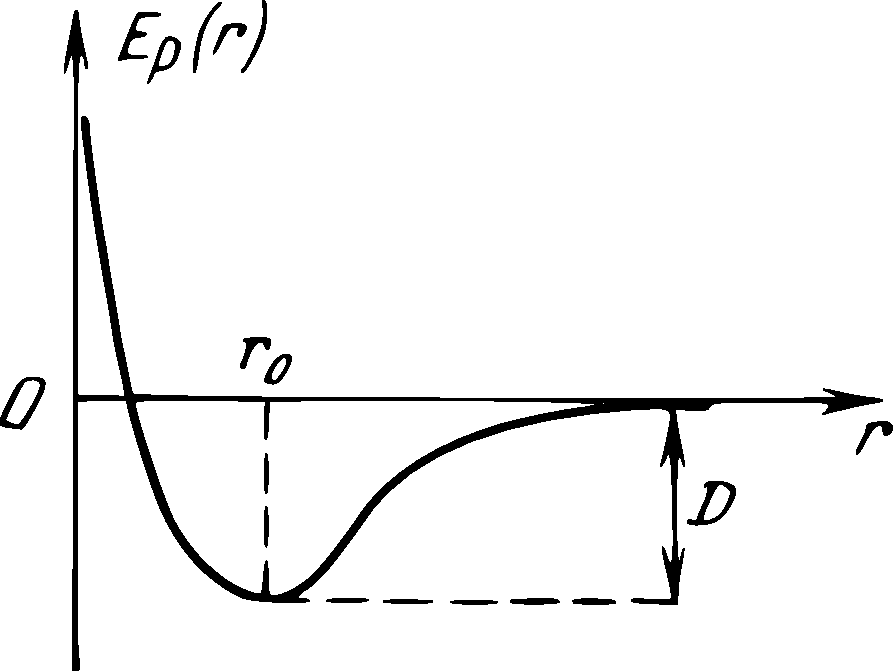
\includegraphics[width=\textwidth]{figs/ch-39/fig-39-03.pdf}
\sidecaption{The potential energy as a function of distance between molecules.\zhcap{势能随分子间距离的变化关系。}\label{fig-39-03}}
\end{marginfigure}

\subsection{}\label{39.4.3} At a certain distance $r_{0}$ between the atoms of a diatomic molecule, the oppositely directed forces of attraction and repulsion counterbalance
each other and their vector sum equals zero. The distance $r_{0}$ corresponds to the minimum mutual (potential) energy $E_{p} (r)$ of the atoms of a diatomic molecule (cf. \ssect{12.1.6}) (\figr{fig-39-03}). The equilibrium interatomic distance $r_{0}$ in a molecule is called the \redem{bond length}, or \redem{distance}. The quantity $D$ is called the \redem{dissociation}, or \redem{bond, energy}. It is numerically equal to the work that must be done to dissociate a molecule into its constituent atoms and to separate them to infinite distances from one another. The dissociation energy is equal to the energy evolved in forming a molecule, but is of opposite sign. Dissociation energy is negative, whereas the energy evolved in forming molecules is positive.
\zhpar{双原子分子中两原子相距为某一距离 $r_{0}$ 时，相互吸引力与排斥力方向相反，二者的矢量和为零。距离 $r_{0}$ 对应于两原子最小的相互（势）能 $E_{p} (r)$（比较 \ssect{12.1.6}）（见\figr{fig-39-03}）。分子中两原子的平衡距离 $r_{0}$ 称为\redem{键长}（或\redem{距离}）。量 $D$ 称为\redem{离解能}（或\redem{键能}），它在数值上等于将分子离解为组成它的原子并使它们彼此相距无穷远所需做的功。离解能在数值上等于形成分子时放出的能量，但符号相反。离解能为负值，而形成分子时放出的能量为正值。}

\subsection{}\label{39.4.4} \redem{Heteropolar (ionic)} molecules are ones formed as the result of the conversion of interacting atoms into oppositely electrically charged and mutually attracting ions \ssect{39.1.1}. This kind of bond between the atoms of a molecule is called a \redem{heteropolar} (or \redem{ionic} or \redem{electrovalent}) bond. The formation of heteropolar molecules is based on the behaviour of atoms with differently filled outer $(s + p)$-subshells, discussed in  \ssect{39.3.9}. Typical heteropolar (ionic) molecules are those of the alkali-halide salts, formed by ions from the elements of the I and VII groups of the periodic system \ssect{39.3.5}. These include: \ce{NaCl} (\ce{Na^{+}Cl^{-}}), \ce{Csl} (\ce{Cs^{+}I^{-}}) and others. Metals of the first group have low ionization potentials $V$ \ssect{39.1.5}, whereas atoms of group VII are characterized by a high \redem{electron affinity}, which is the amount of energy released when an electron is attached to a metalloid atom. The transition of an electron from a metal atom to a metalloid atom leads to the formation of ions, each of which has a stable eight-electron $(s + p)$-subshell \ssect{39.3.9}. As a result, a stable heteropolar (ionic) molecule is formed.
\zhpar{\redem{异极（离子）分子}是由相互作用的原子转变为带相反电荷、相互吸引的离子而形成的分子 \ssect{39.1.1}。分子中原子之间的这种化学键称为\redem{异极（离子）键}，亦称\redem{电价键}。异极分子的形成基于外层 $(s + p)$ 支壳层填充情况不同的原子的性质，见 \ssect{39.3.9}。典型的异极（离子）分子是碱卤盐的分子，它们由元素周期表中第 I 族和第 VII 族元素的离子构成 \ssect{39.3.5}，例如 \ce{NaCl}（\ce{Na^{+}Cl^{-}}）、\ce{Csl}（\ce{Cs^{+}I^{-}}）等。第一族金属的电离势 $V$ 较低 \ssect{39.1.5}，而第 VII 族原子则具有较高的\redem{电子亲和能}，即电子附着到非金属原子上时所放出的能量。电子从金属原子转移到非金属原子上，形成各自具有稳定八电子 $(s + p)$ 支壳层的离子，结果形成稳定的异极（离子）分子。}
\clearpage
\subsection{}\label{39.4.5} \redem{Homopolar (atomic)} molecules are ones formed by the mutual attraction of neutral atoms. The chemical bond of the atoms of a homopolar molecule is said to be covalent. A covalent bond lias the property of being saturated (saturation of a covalent bond), which is manifested as the definite valency of the atoms.
\zhpar{\redem{同极（原子）分子}是由中性原子相互吸引而形成的分子。同极分子中原子间的化学键称为共价键。共价键具有饱和性（共价键的饱和性），表现为原子具有确定的化合价。}

An atom of hydrogen can be bound to only one other atom, and
an atom of carbon to no more that four other atoms. The simplest molecule with a covalent bond is the hydrogen molecule \ce{H2}; it consists of two electrons and two nuclei-protons. 
\zhpar{氢原子只能与一个其他原子结合，而碳原子最多可与四个其他原子结合。最简单的具有共价键的分子是氢分子 \ce{H2}，它由两个电子和两个质子（即两个原子核）组成。}

The basis of the quantum-mechanical explanation of the covalent bond in the \ce{H2} molecule is the indistinguishability of identical particles, e.g. the electrons in a hydrogen molecule (see also \ssect{41.1.2}). The electrons in the \ce{H2} molecule, each of which ``belongs'' to a definite nucleus, can be interchanged and this still leads to the same system: an \ce{H2} molecule consisting of two electrons and two nuclei. The indistinguishability of electrons leads to the occurrence of a special \redem{quantum-mechanical exchange interaction} between two identical electrons. This interaction consists in the electron of each of the atoms in the hydrogen molecule spending a certain part of its time at the nucleus of the other atom. This constitutes the bond between the two atoms forming the molecule. It follows from quantum-mechanical calculations that when two hydrogen atoms approach each other to a distance commensurable with the Bohr radius \ssect{39.1.9}, and under the condition that the spins of the electrons in the atoms are antiparallel
\ssect{26.1.3}, the two atoms attract each other and a stable
\ce{H2} molecule is formed. With parallel spins of the electrons, the two atoms of hydrogen repel each other, and no molecule of hydrogen
is formed.
\zhpar{对氢分子 \ce{H2} 中共价键进行量子力学解释的基础，是全同粒子的不可分辨性，例如氢分子中的电子（另见 \ssect{41.1.2}）。\ce{H2} 分子中的每个电子各“属于”某一确定的原子核，两个电子可以互换，而所得体系仍然相同，即仍是由两个电子和两个原子核组成的 \ce{H2} 分子。电子的不可分辨性导致两个全同电子之间存在一种特殊的\redem{量子力学交换相互作用}。这种相互作用表现为：氢分子中每个原子的电子都要花费一定的时间停留在另一个原子核附近。这就构成了形成分子的两个原子之间的化学键。量子力学计算表明，当两个氢原子相互接近到与玻尔半径 \ssect{39.1.9} 相当的距离，且两原子中电子的自旋反平行 \ssect{26.1.3} 时，两原子相互吸引，形成稳定的 \ce{H2} 分子。若电子自旋平行，两个氢原子则相互排斥，不能形成氢分子。}

\section{Optical Properties of Molecules. Molecular Spectra}
\label{sec-39.5} 
\zhtitle{分子的光学性质。分子光谱}


\subsection{}\label{39.5.1} Owing to their specific appearance, the spectra of molecules, or \redem{molecular spectra}, are called \redem{band spectra}. They consist of a set of more or less wide bands formed of closely spaced spectral lines. Bands are observed in molecular spectra in the infrared, visible
and ultraviolet ranges of the scale of electromagnetic waves,
\ssect{31.4.3}. Closely spaced bands form a \redem{group of bands}. Several groups of bands are observed for the simplest diatomic molecules.
\zhpar{由于外观特殊，\redem{分子光谱}称为\redem{带状光谱}。它由一组或宽或窄的谱带组成，每个谱带则由间距很小的谱线构成。在电磁波标度的红外、可见光和紫外区域都可以观察到分子光谱中的谱带 \ssect{31.4.3}。彼此靠近的谱带构成一个\redem{谱带组}。对于最简单的双原子分子，可观察到若干个谱带组。}

Continuous broad emission (or absorption) bands are observed in the visible and ultraviolet regions of the spectra of polyatomic complex molecules.
\zhpar{在复杂多原子分子的光谱中，可见光和紫外区域观察到连续的宽发射（或吸收）谱带。}

\subsection{}\label{39.5.2} As in the spectra of atoms \ssect{39.1.3}, a separate spectral line in a molecular spectrum appears as a result of a change in the energy of a molecule. The total energy $E^{m}$ of a molecule can be presented as the sum of the following parts, assumed independent in a first approximation:
\zhpar{与原子光谱一样 \ssect{39.1.3}，分子光谱中的单条谱线是分子能量变化的结果。在一级近似下，可将分子的总能量 $E^{m}$ 看作下列各部分之和，并假定它们彼此独立：}
\begin{equation*}%
E^{m} = E^{m}_{t} + E^{m}_{e} + E^{m}_{v} + E^{m}_{r} + E^{m}_{n}, 
\end{equation*}
where $E^{m}_{t}$ is the energy of translational motion of the centre of mass \ssect{2.3.3} of the molecule, $E^{m}_{e}$ is the energy of motion of the electrons in the molecule's atoms, $E^{m}_{v}$ is the energy of vibrational motion about their equilibrium positions of the nuclei in the molecule's
atoms, $E^{m}_{r}$ is the energy of rotary motion of the molecule as a whole, and $E^{m}_{n}$ is the energy of the nuclei in the molecule's atoms. The energy $E^{m}_{t}$ is not quantized \ssect{38.4.3} and its-change cannot lead to the production of a molecular spectrum; the effect of $E^{m}_{n}$ on the molecular spectrum can be neglected in a first approximation.
\zhpar{式中 $E^{m}_{t}$ 为分子质心 \ssect{2.3.3} 平动的能量，$E^{m}_{e}$ 为分子中原子内电子运动的能量，$E^{m}_{v}$ 为分子中原子核在其平衡位置附近振动的能量，$E^{m}_{r}$ 为分子整体转动的能量，$E^{m}_{n}$ 为分子中原子核的能量。能量 $E^{m}_{t}$ 不是量子化的 \ssect{38.4.3}，其变化不能产生分子光谱；在一级近似下，可以忽略 $E^{m}_{n}$ 对分子光谱的影响。}

The energy $E^{'m}$ in of the molecule, whose change governs
the molecular spectrum, constitutes the sum of three components:
\zhpar{决定分子光谱的分子能量 $E^{'m}$ 由下列三个分量之和组成：}
\begin{equation*}%
E^{'m} = E^{m}_{e} + E^{m}_{v} + E^{m}_{r}.
\end{equation*}

\subsection{}\label{39.5.3} According to the Bohr frequency condition \ssect{39.1.6}, the frequency $\nu$ of the photon emitted by the molecule when its energy state changes is equal to 
\zhpar{根据玻尔频率条件 \ssect{39.1.6}，分子能态变化时所发射光子的频率 $\nu$ 等于：}
\begin{equation*}%
\nu = \frac{\Delta E^{'m}}{h} = \frac{\Delta E^{m}_{e}}{h} + \frac{\Delta E^{m}_{v}}{h} + \frac{\Delta E^{m}_{r}}{h},
\end{equation*}
where $\Delta E^{m}_{e}$, $\Delta E^{m}_{v}$ and $\Delta E^{m}_{r}$ are the changes in the corresponding parts of the energy $E^{'m}$, which assume discrete quantized values.
\zhpar{式中 $\Delta E^{m}_{e}$、$\Delta E^{m}_{v}$ 和 $\Delta E^{m}_{r}$ 分别为能量 $E^{'m}$ 相应部分的变化量，它们取分立的量子化值。}

The production of closely spaced lines, forming bands at various parts of the spectrum, is explained by the fact that
\zhpar{光谱中形成谱带的彼此靠近的谱线之所以产生，可由下列事实解释：}
\begin{equation*}%
E^{m}_{r}\ll  E^{m}_{v} \ll E^{m}_{e} .
\end{equation*}

In the far-infrared region of the spectrum (wavelengths of the
order of 0.1 to 1~mm), the transition of the molecule from one rotational energy level to another produces spectral lines of a \redem{rotation spectrum}.
\zhpar{在远红外区域（波长约为 0.1 至 1~mm），分子从一个转动能级跃迁到另一个转动能级，产生\redem{转动光谱}的谱线。}

\begin{marginfigure}%[-3cm] 
\centering
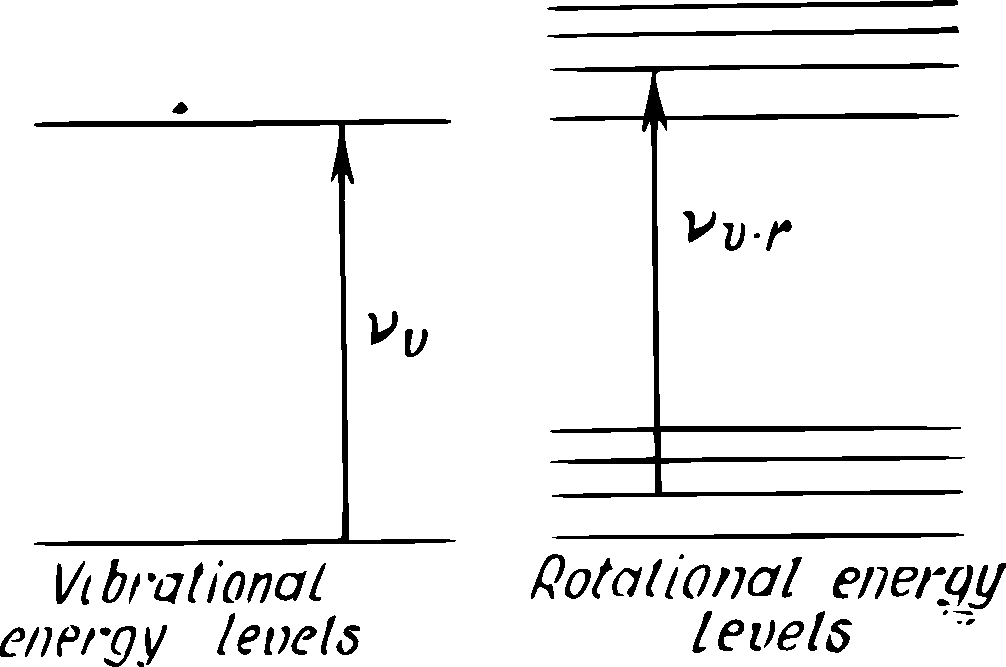
\includegraphics[width=\textwidth]{figs/ch-39/fig-39-04.pdf}
\sidecaption{Vibrational and rotational energy levels of molecules.\zhcap{分子的振动能级和转动能级。}\label{fig-39-04}}
\end{marginfigure}

\subsection{}\label{39.5.4} In the infrared region of the spectrum (wavelengths from one to several dozen micrometres), transitions of molecules between vibrational energy levels produce the lines of the \redem{vibrational spectrum} of the molecule. Upon changes in the vibrational energy levels of the molecule, its rotational energy levels are also changed at the same time. Hence, transitions of molecules between vibrational
levels are vibrational-rotational transitions, producing
a \redem{vibrational-rotational spectrum} with the frequencies $\nu_{vr}$ (\figr{fig-39-04}). This spectrum consists of groups of closely spaced lines determined by the fact that the given vibrational transition is accompanied by rotational transitions.
\zhpar{在红外区域（波长从一微米到几十微米），分子在振动能级之间的跃迁产生分子的\redem{振动光谱}谱线。分子的振动能级发生变化时，其转动能级也同时改变。因此，分子在振动能级之间的跃迁是振动-转动跃迁，产生频率为 $\nu_{vr}$ 的\redem{振转光谱}（见\figr{fig-39-04}）。这种光谱由一组组彼此靠近的谱线构成，原因在于给定的振动跃迁总伴随着转动跃迁。}

\begin{marginfigure}%[-3cm] 
\centering
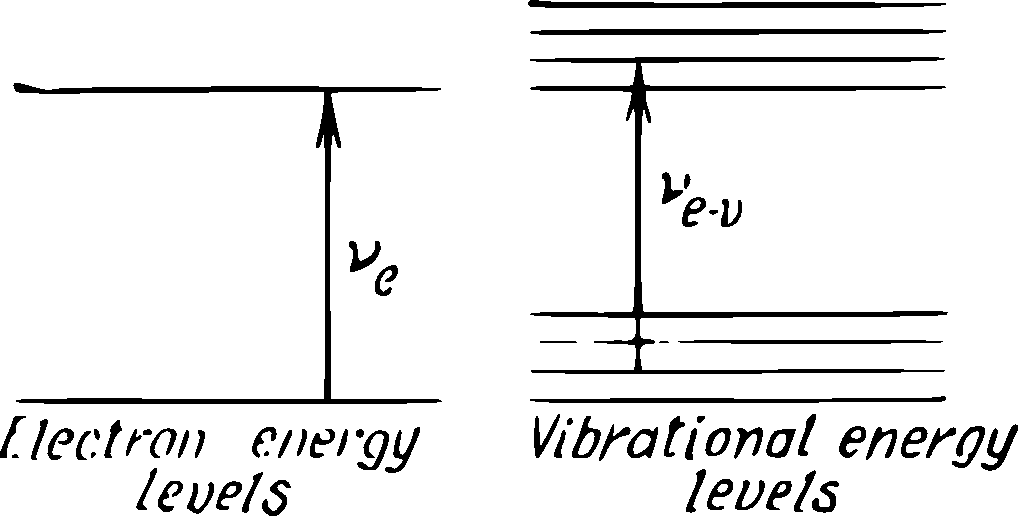
\includegraphics[width=\textwidth]{figs/ch-39/fig-39-05.pdf}
\sidecaption{Vibrational and electron energy levels of molecules.\zhcap{分子的振动能级和电子能级。}\label{fig-39-05}}
\end{marginfigure}

\subsection{}\label{39.5.5} The visible and ultraviolet regions of the spectrum are produced as a result of transitions of the molecule between the various electron energy levels. Each electron energy level corresponds to various possible vibrations of the nucleus in the molecule, i.e. to a set of vibrational energy levels. Transitions between electron-vibrational levels lead to the production of an \redem{electron-vibrational spectrum} of the molecule, characterized by the frequencies $\nu_{ev}$ of the various lines (\figr{fig-39-05}). Since each vibrational energy state corresponds to a system of rotational levels \ssect{39.5.4},
each electron-vibrational transition corresponds to a certain
band. The whole electron-vibrational spectrum of the molecule in the visible and nearby regions consists of a system of several groups of bands.
\zhpar{分子光谱的可见光区和紫外区，是分子在各种电子能级之间跃迁所产生的。每个电子能级对应于分子中原子核的各种可能振动，即对应于一组振动能级。电子-振动能级之间的跃迁产生分子的\redem{电子-振动光谱}，其特征为各谱线的频率 $\nu_{ev}$（见\figr{fig-39-05}）。由于每个振动能态对应于一组转动能级 \ssect{39.5.4}，每一个电子-振动跃迁都对应于一个确定的谱带。分子在可见光及邻近区域的整个电子-振动光谱由若干谱带组构成。}

\section{Raman Scattering of Light}
\label{sec-39.6} 
\zhtitle{光的拉曼散射}

\subsection{}\label{39.6.1} \redem{Raman scattering of light}\sidenote{Commonly called combination scattering in the Soviet literature.}, or the Raman effect, refers to the shifted frequencies $\nu_{s}$ and $\nu_{a}$ observed, along with the frequency $\nu_{0}$ of the source of radiation, in the spectrum of light scattered by a solid or liquid body. 
\zhpar{\redem{光的拉曼散射}（或拉曼效应）是指：在固体或液体散射光的光谱中，除光源频率 $\nu_{0}$ 外，还观察到频率发生移动的 $\nu_{s}$ 和 $\nu_{a}$。}
\zhpar{注：该现象在苏联文献中通常称为组合散射。}

A spectral line with the frequency $\nu_{s} = \nu_{0} - \nu$ is called a \redem{Stokes (red) line}; one with the frequency $\nu_{s} = \nu_{0} + \nu$ is called an \redem{anti-Stokes (violet) line}. The set of lines with the frequencies $\nu_{s}$ and $\nu_{a}$ form the Raman spectrum of the molecule, containing red and violet \redem{satellites with the frequency} $\nu_{0}$. The intensity of the violet satellites is less than that of the red ones, but increases with the temperature. The intensity of the red satellites is practically independent of the temperature.
\zhpar{频率为 $\nu_{s} = \nu_{0} - \nu$ 的谱线称为\redem{斯托克斯（红）线}；频率为 $\nu_{s} = \nu_{0} + \nu$ 的谱线称为\redem{反斯托克斯（紫）线}。频率为 $\nu_{s}$ 和 $\nu_{a}$ 的谱线构成分子的拉曼光谱，其中包括与频率 $\nu_{0}$ 相伴的红色和紫色\redem{伴线}。紫色伴线的强度小于红色伴线，但随温度升高而增强。红色伴线的强度几乎与温度无关。}

\subsection{}\label{39.6.2} The quantum-mechanical explanation of the Raman scattering phenomenon consists in an analysis of the interaction between a photon of incident light having the frequency $\nu_{0}$ and a molecule at the ground vibrational energy level with the energy $E^{m}_{1v}$. If, as a result of the interaction with the photon, the molecule is moved to higher vibrational energy level with the energy $E^{m}_{2V} > E^{m}_{1V}$, the energy $\Delta E^{m} = E^{m}_{2V} - E^{m}_{1V}$ required for this purpose is borrowed from the incident light. A photon with the energy $h \nu_{0}$ is absorbed and, in its place, a photon is produced with lower frequency $\nu$ and an energy equal to $h \nu = h \nu_{0} - \Delta E^{m}$.
\zhpar{拉曼散射现象的量子力学解释，在于分析频率为 $\nu_{0}$ 的入射光子与处于基态振动能级（能量为 $E^{m}_{1v}$）的分子之间的相互作用。若由于相互作用，分子被激发到能量较高的振动能级 $E^{m}_{2V} > E^{m}_{1V}$，则为此所需的能量 $\Delta E^{m} = E^{m}_{2V} - E^{m}_{1V}$ 取自入射光。能量为 $h \nu_{0}$ 的光子被吸收，同时产生一个频率较低、能量为 $h \nu = h \nu_{0} - \Delta E^{m}$ 的光子。}

At this the frequency $\nu$ appears in the scattered light. It equals 
\zhpar{此时，散射光中出现频率 $\nu$，它等于：}
\begin{equation*}%
\nu_{s} = \nu_{0} - \frac{\Delta E^{m}}{h},
\end{equation*}
and corresponds to the frequency of a red satellite. The whole set of red satellites are produced in transitions of the molecule to various excited vibrational energy states.
\zhpar{该频率对应于红色伴线。全部红色伴线都是分子跃迁到各激发振动能态时产生的。}

\subsection{}\label{39.6.3} If a molecule at the vibrational energy level with the energy $E^{m}_{2V}$ \ssect{39.6.2} moves, due to interaction with a photon having the energy $h \nu_{0}$, to an energy state with less energy $(E^{m}_{1v})$, a violet satellite of the frequency $\nu_{a}$ is produced in the scattered light spectrum. This frequency
\zhpar{若分子处于能量为 $E^{m}_{2V}$ 的振动能级上（见 \ssect{39.6.2}），在与能量为 $h \nu_{0}$ 的光子相互作用后跃迁到能量较低的状态 $(E^{m}_{1v})$，则散射光谱中将产生频率为 $\nu_{a}$ 的紫色伴线。该频率为：}
\begin{equation*}%
\nu_{a} = \nu_{0} + \frac{\Delta E^{m}}{h},
\end{equation*}
where $\Delta E^{m} = \Delta E^{m}_{2V} - \Delta E^{m}_{1V}$.
\zhpar{式中 $\Delta E^{m} = \Delta E^{m}_{2V} - \Delta E^{m}_{1V}$。}

The probability of Raman scattering with an increase in frequency is less than the same scattering with a reduction in frequency. This is due to the fact that the number of molecules at the higher energy levels is less than the number at the lower levels. Consequently, the intensity of violet satellites is less than that of the red ones. When the temperature is raised, the molecule population of the upper energy levels increases, as does the intensity of the violet satellites. The number of molecules in the ground state changes only slightly upon heating. Therefore, the intensity of the red satellites, remains practically unchanged as the  temperature is raised.
\zhpar{频率升高的拉曼散射概率小于频率降低的同类散射概率。这是因为处于较高能级的分子数少于处于较低能级的分子数。因此，紫色伴线的强度小于红色伴线的强度。升高温度时，处于较高能级的分子数增加，紫色伴线的强度也随之增强。加热时，处于基态的分子数变化很小，因此红色伴线的强度实际上保持不变。}

\section{Luminescence. X rays}
\label{sec-39.7} 
\zhtitle{发光。X 射线}


\subsection{}\label{39.7.1} \redem{Luminescence} is the radiation of light by bodies at a temperature $T$, which is over and above the thermal radiation \ssect{36.1.1} at this temperature. The duration of luminescence substantially exceeds the periods of radiation of atomic systems. Depending upon the method applied to excite the luminescent glow, distinction is made between cathodoluminescence, electroluminescence, photoluminescence and chemiluminescence. Luminescent substances are called \redem{luminophors}.
\zhpar{\redem{发光}是物体在温度 $T$ 下发出的光，它超出了该温度下的热辐射 \ssect{36.1.1}。发光的持续时间远大于原子系统辐射的周期。根据激发发光的方法不同，可区分为阴极射线发光、电致发光、光致发光和化学发光。发光物质称为\redem{发光体}。}

\subsection{}\label{39.7.2} Luminescent radiation is a nonequilibrium one (cf. \ssect{36.1.2}) and is caused by a comparatively small number of \redem{luminescence centres} --  atoms, molecules or ions -- put into an excited state by the source of luminescence. The return of the excited centre to its ground or less excited state is accompanied by \redem{luminescent radiation}. The duration of this radiation is determined by the duration of the excited state, which depends on the properties of not only the radiating centres, but of the medium surrounding them as well. The duration of a metastable excited state can reach \SI{d-4}{\second}, thereby correspondingly increasing the duration of the luminescence.
\zhpar{发光辐射是非平衡辐射（比较 \ssect{36.1.2}），它是由数量相对较少的\redem{发光中心}（即被光源激发到激发态的原子、分子或离子）所引起的。激发中心回到基态或较低激发态时，便伴随着\redem{发光辐射}。这种辐射的持续时间取决于激发态的持续时间，而激发态的持续时间不仅取决于辐射中心的性质，还取决于包围它们的介质的性质。亚稳激发态的持续时间可达 \SI{d-4}{\second}，从而相应地延长了发光的持续时间。}

\subsection{}\label{39.7.3} Luminescence that immediately ceases together with the action of the glow exciting source is called \redem{fluorescence}. Luminescence that persists long after the action of the glow exciting source has ceased to act is called \redem{phosphorescence}. 
\zhpar{随激发光源作用的停止而立即停止的发光称为\redem{荧光}。在激发光源停止作用后仍然持续很长时间的发光称为\redem{磷光}。}

The phenomenon of fluorescence is associated with the transitions of atoms, molecules or ions from ordinary excited states with a duration of the order of \SI{d-8}{\second}to the ground state. Phosphorescence, which provides for prolonged glow, is due to the transition of luminescence centres from metastable states to the ground state \ssect{39.7.2}. The subdivision of luminescence into fluorescence and phosphorescence is arbitrary; it is sometimes difficult to establish a time-based boundary between them.
\zhpar{荧光现象与原子、分子或离子从通常的激发态（持续时间约为 \SI{d-8}{\second}）跃迁到基态有关。磷光能够持续较长时间，是由于发光中心从亚稳态跃迁到基态所致 \ssect{39.7.2}。将发光划分为荧光和磷光是任意的，有时很难确定二者之间的时间界限。}

\subsection{}\label{39.7.4} The excitation of luminescence by moans of an electron beam is feasible provided that the kinetic energy of a bombarding electron satisfies the inequality
\zhpar{利用电子束激发发光是可行的，条件是入射电子的动能满足下列不等式：}
\begin{equation*}%
\frac{mv^{2}}{2} \geqslant E_{e} - E_{g},
\end{equation*}
where $E_{e}$ and $E_{g}$ are the total energies of the luminescent particle in the excited and ground states.
\zhpar{式中 $E_{e}$ 和 $E_{g}$ 分别为发光粒子处于激发态和基态时的总能量。}

\subsection{}\label{39.7.5} \redem{Photoluminescence} is excited by electromagnetic radiation in the visible or ultraviolet ranges and complies with the \redem{Stokes
law}: the wavelength of photoluminescence is usually longer than that of the exciting light. The quantum-mechanical basis for the Stokes law is that in the absorption of a photon of exciting light with the energy $h \nu$, a photon with the energy $h \nu_{\mathrm{lum}}$, less than $h \nu$, is produced. The surplus energy $h \nu - h \nu_{\mathrm{lum}} = E^{m}$, where $E^{m}$ is
energy expended on various processes except photoluminescence.
\zhpar{\redem{光致发光}由可见光或紫外区域的电磁辐射激发，并遵循\redem{斯托克斯定律}：光致发光的波长通常比激发光的波长长。斯托克斯定律的量子力学基础在于：吸收一个能量为 $h \nu$ 的激发光光子时，产生一个能量为 $h \nu_{\mathrm{lum}}$ 的光子，且该能量小于 $h \nu$。剩余能量 $h \nu - h \nu_{\mathrm{lum}} = E^{m}$ 用于光致发光以外的各种过程，其中 $E^{m}$ 即为这些过程所消耗的能量。}

As a rule, $E_{m} > 0$ and $\nu_{\mathrm{lum}} < \nu$, i.e.  $\lambda_{\mathrm{lum}} > \lambda$ in accordance with the Stokes law. Sometimes, \redem{anti-Stokes luminescent radiation} is observed. It complies with a condition that is the opposite of
the Stokes law, i.e. $\lambda_{\mathrm{lum}} < \lambda$. This occurs when a definite part of the energy of thermal motion of the particles of the luminescent substance is added to the energy $h \nu$ of the photon that excites the luminescence. Thus
\zhpar{通常 $E_{m} > 0$，$\nu_{\mathrm{lum}} < \nu$，即 $\lambda_{\mathrm{lum}} > \lambda$，符合斯托克斯定律。有时也观察到\redem{反斯托克斯发光辐射}，它满足与斯托克斯定律相反的条件，即 $\lambda_{\mathrm{lum}} < \lambda$。当发光物质中粒子热运动能量的一部分加到激发发光的光子能量 $h \nu$ 上时，就会出现这种情况。于是有：}
\begin{equation*}%
h \nu_{\mathrm{lum}} = h \nu+ akT,
\end{equation*}
where $a$ is a factor depending upon the nature of the luminescent substance, $k$ is Boltzmann's constant \ssect{8.4.5}, and $T$ is the absolute temperature.
\zhpar{式中 $a$ 为取决于发光物质性质的因子，$k$ 为玻尔兹曼常量 \ssect{8.4.5}，$T$ 为热力学温度。}

\subsection{}\label{39.7.6} \redem{Photoluminescent energy efficiency} is the ratio of the energy of luminescent radiation to the energy from the source absorbed under steady-state conditions by the luminophor.
\zhpar{\redem{光致发光能量效率}是发光辐射的能量与发光体在稳定状态下从光源吸收的能量之比。}

The \redem{quantum yield of photoluminescence} is the ratio of the number of photons of photoluminescent radiation to the number of photons of the exciting light, the latter having constant energy. \redem{Vavilov's law} states that the photoluminescent energy efficiency increases proportionally to the wavelength $\lambda$ of the absorbed radiation. Then,
after reaching a maximum value in the wavelength range from $\lambda$ to $\lambda_{\mathrm{max}}$, drops rapidly to zero upon a further increase in wavelength. With an increase in the wavelength of the exciting light of given energy, there is an increase in the number of photons contained in the given energy of primary radiation. Each of these photons can produce a photon of the energy $h \nu_{\mathrm{lum}}$. Therefore, the photoluminescent energy efficiency increases with the wavelength $\lambda$. The sharp drop in energy efficiency at $\lambda = \lambda_{\mathrm{max}}$ indicates that photons with the frequency less than $\nu_{\mathrm{min}} = c /\lambda_{\mathrm{max}}$ cannot excite the particles of the luminophor.
\zhpar{\redem{光致发光量子产额}是光致发光辐射的光子数与激发光光子数之比，后者的能量为恒定值。\redem{瓦维洛夫定律}指出：光致发光能量效率随所吸收辐射的波长 $\lambda$ 成比例增加，并在波长从 $\lambda$ 到 $\lambda_{\mathrm{max}}$ 的范围内达到最大值，随后在波长进一步增大时迅速降至零。在给定能量下，随着激发光波长的增加，该能量中所包含的光子数增多。这些光子中的每一个都可以产生一个能量为 $h \nu_{\mathrm{lum}}$ 的光子。因此，光致发光能量效率随波长 $\lambda$ 的增加而增大。在 $\lambda = \lambda_{\mathrm{max}}$ 处能量效率的急剧下降表明，频率小于 $\nu_{\mathrm{min}} = c /\lambda_{\mathrm{max}}$ 的光子不能激发发光体中的粒子。}

\subsection{}\label{39.7.7} \redem{$X$-rays} are electromagnetic waves with a wavelength from 0.01 to \SI{800}{\angstrom} that are produced by braking high-speed electrons by a substance. There are two types of short-wave $X$ rays.
\zhpar{\redem{$X$ 射线}是波长为 0.01 至 \SI{800}{\angstrom} 的电磁波，由物质使高速电子减速而产生。短波 $X$ 射线有两种类型。}

At electron energies, not exceeding a certain critical value that depends upon the substance in which the electrons are braked, \redem{white}, or \redem{continuous, $X$ rays} are produced. It is radiated by braked electrons and has a continuous spectrum, bounded on the short-wavelength side by a certain boundary $\lambda_{\mathrm{min}}$, called the \redem{continuous-spectrum boundary}. The boundary wavelength $\lambda_{\mathrm{min}}$ depends upon the kinetic energy $E_{k}$ of the electrons that produce the bremsstrahlung and is reduced with an increase in the kinetic energy $E_{k}$. The existence of $\lambda_{\mathrm{min}}$ is explained by the fact that the maximum energy frvmax of a photon of $X$ rays, produced at the expense of the energy of the electron, cannot exceed $E_{k}$. Thus
\zhpar{当电子能量不超过某一临界值（该临界值取决于使电子减速的物质）时，产生\redem{白色}或\redem{连续 $X$ 射线}。它由减速电子辐射产生，具有连续谱，在短波一侧以某一边界 $\lambda_{\mathrm{min}}$ 为界，称为\redem{连续谱边界}。边界波长 $\lambda_{\mathrm{min}}$ 取决于产生韧致辐射的电子动能 $E_{k}$，并随动能 $E_{k}$ 的增大而减小。$\lambda_{\mathrm{min}}$ 的存在可以这样解释：由电子能量转化而产生的 $X$ 射线光子的最大能量（即 $h \nu_{\mathrm{max}}$）不能超过 $E_{k}$。于是有：}
\begin{equation*}%
h \nu_{\mathrm{max}} = E_{k}.
\end{equation*}
Consequently, 
\zhpar{由此可得：}
\begin{equation*}%
\lambda_{\mathrm{min}} = \frac{c}{\nu_{\mathrm{max}}} = \frac{c h}{E_{k}}.
\end{equation*}
 Making use of data on the values of $E_{k}$ and $\lambda_{\mathrm{min}}$, this formula enables Planck's constant (Appendix~II) to be determined. In its time this method was one of the most accurate and reliable ones.
\zhpar{利用 $E_{k}$ 和 $\lambda_{\mathrm{min}}$ 的数据，可由该公式确定普朗克常量（见附录 II）。在当时，这种方法是最精确、最可靠的方法之一。}

\subsection{}\label{39.7.8} The second type of $X$ rays, \redem{characteristic $X$ radiation} of atoms of matter, has a line spectrum. It is an individual characteristic of a substance and does not change when the substance enters a chemical compound. It follows that, contrary to optical spectra,
characteristic $X$ rays are associated with processes in the deep-lying filled inner electron shells of atoms \ssect{39.3.6}, which undergo no changes in chemical reactions of the atoms. \redem{Line $X$ ray spectra} consist of lines composing several series. The same types of line series are observed in various elements, differing only in that the like series of lines in the heavier elements are shifted toward the
side of shorter wavelengths.
\zhpar{第二种类型的 $X$ 射线是物质原子的\redem{特征 $X$ 辐射}，它具有线状谱。这种辐射是物质的个性特征，物质参与化学化合时它不发生改变。由此可见，与光学光谱不同，特征 $X$ 射线与原子中深层已填满的内电子壳层中的过程有关 \ssect{39.3.6}，而这些壳层在原子的化学反应中不发生变化。\redem{线状 $X$ 射线谱}由若干谱线系组成。同类谱线系在不同元素中都能观察到，其差别仅在于较重元素中相应谱线系向较短波长一侧移动。}

\subsection{}\label{39.7.9} In the order of increasing wavelengths, the series of characteristic $X$ rays are called the $K$-, $L$- $M$-, and $N$-series. As an electron is removed from one of the inner shells of an atom with the nuclear charge $Ze$, the vacant space is occupied by an electron from a shell farther from the nucleus and an $X$-ray photon is emitted. Thus, after removing an electron from the $A$-shell, the filling of the vacancy by electrons from $L$-, $M$- and other shells, produces the $K_{\alpha}$-, $K_{\beta}$- and $K_{\gamma}$-lines that form the $K$-series,
\zhpar{按波长增大的顺序，特征 $X$ 射线的各谱线系依次称为 $K$ 系、$L$ 系、$M$ 系和 $N$ 系。当核电荷为 $Ze$ 的原子的某一内层电子被移走后，空位由离核更远的壳层中的电子填补，同时发射一个 $X$ 射线光子。例如，从 $K$ 壳层移走电子后，由 $L$、$M$ 等壳层中的电子填补空位，产生构成 $K$ 系的 $K_{\alpha}$、$K_{\beta}$ 和 $K_{\gamma}$ 谱线。}

The frequency $\nu$ of the lines of characteristic $X$ rays can be found by \redem{Mosley's law}:
\zhpar{特征 $X$ 射线谱线的频率 $\nu$ 可由\redem{莫塞莱定律}求得：}
\begin{equation*}%
\sqrt{\nu} = a(Z - b),
\end{equation*}
where $a$ is a constant for the given series of lines (in $s^{-1/2}$), and $b$ is the screening constant. This constant means that an electron, accomplishing a transition corresponding to a certain line, is subject, not to the whole charge $Ze$ of the nucleus, but to the charge $(Z - b) e$, which has been weakened by the screening action of other electrons.
\zhpar{式中 $a$ 为该谱线系的常量（单位为 $s^{-1/2}$），$b$ 为屏蔽常量。屏蔽常量的含义是：与某一谱线相对应的跃迁所涉及的电子，所受到的不是原子核的全部电荷 $Ze$，而是被其他电子屏蔽而减弱了的电荷 $(Z - b) e$。}

\section{Stimulated Emission of Radiation. Lasers}
\label{sec-39.8} 
\zhtitle{受激辐射。激光器}


\subsection{}\label{39.8.1} An atom located in an electromagnetic field at an excited energy level can, with a certain probability, be transferred by the effect of the field to a lower energy state. It is as if the electromagnetic field ``tumbles'' the atom down from its excited level to the ground state or only to a less excited state. Such a transition is accompanied by \redem{stimulated (induced) radiation} of the substance, produced by the action of an electromagnetic wave on it.
\zhpar{处于电磁场中激发能级上的原子，在一定概率下可在场的作用下跃迁到较低能态。这就好像电磁场把原子从激发能级“推落”到基态，或推落到较低的激发态。这种跃迁伴随着物质的\redem{受激（感生）辐射}，它是由电磁波作用于物质而产生的。}

\subsection{}\label{39.8.2} From the viewpoint of wave optics \ssect{32.1.1} the phenomenon of stimulated emission of radiation means that as the electromagnetic wave passes through a substance its intensity \ssect{31.2.4} is
increased, i.e. \redem{negative absorption of light occurs}. But the frequency \ssect{30.2.5} of the wave, direction of its propagation, its phase \ssect{30.2.5} and polarization \ssect{31.1.7} remain unchanged. Stimulated emission
of radiation is \redem{strictly coherent} \ssect{30.5.1} to the electromagnetic wave passing through the substance and producing the emission.
\zhpar{从波动光学的观点看，受激辐射现象意味着：电磁波穿过物质时其强度 \ssect{31.2.4} 增大，即发生\redem{负吸收}。但是，电磁波的频率 \ssect{30.2.5}、传播方向、相位 \ssect{30.2.5} 和偏振 \ssect{31.1.7} 保持不变。受激辐射与穿过物质并产生它的电磁波\redem{严格相干} \ssect{30.5.1}。}

\subsection{}\label{39.8.3} From the quantum-mechanical point of view, the coherence mentioned in \ssect{39.8.2} means that the new photon, produced as a result of the stimulated emission, in no way differs from the photon it was produced by. The new photon, produced in stimulated emission, strengthens the light passing through the medium. As is shown in \figr{fig-39-06}~(b), the process of stimulated emission leads to the production of two photons with the energy $h \nu$ in place of
one such photon. But, in addition to stimulated emission, absorption of light also occurs. As a result of the absorption of a photon by an atom at the energy level $E_{1}$ the photon disappears and the atom moves to the energy level $E_{2}$ (\figr{fig-39-06}~(a)). This process reduces the intensity of the light that passes through the substance.
\zhpar{从量子力学的观点看，上面提到的相干性意味着：受激辐射所产生的新光子与产生它的光子完全没有区别。受激辐射产生的新光子加强了穿过介质的光。如\figr{fig-39-06}（b）所示，受激辐射过程使一个此类光子变为两个能量均为 $h \nu$ 的光子。但是，除受激辐射外，光的吸收也会发生。光子被能级 $E_{1}$ 上的原子吸收后，光子消失，原子跃迁到能级 $E_{2}$（见\figr{fig-39-06}（a））。这一过程使穿过物质的光的强度减弱。}

\begin{figure}%[-3cm] 
\centering
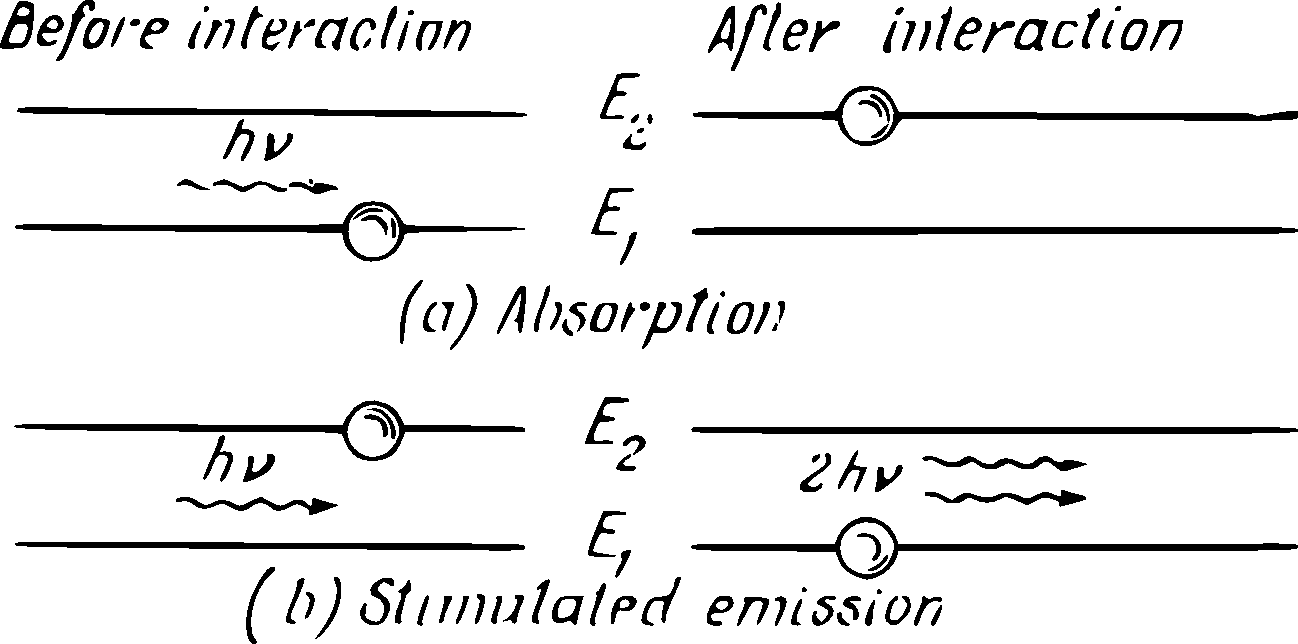
\includegraphics[width=0.8\textwidth]{figs/ch-39/fig-39-06.pdf}
\sidecaption{Absorption and simulated emission of radiation.\zhcap{吸收和受激辐射。}\label{fig-39-06}}
\end{figure}


\subsection{}\label{39.8.4} A medium is said to be active if in it the intensity of transmitted light increases. This indicates that in an active medium the process of stimulated emission predominates over the process of light absorption. Otherwise, when the chief role is played by the absorption of light, the medium weakens the radiation passing through it. An active medium is also called one with negative absorption \ssect{39.8.1}.
\zhpar{若介质中透射光的强度增大，则称该介质为活性介质。这表明在活性介质中，受激辐射过程占优于光的吸收过程。反之，若光的吸收起主要作用，则介质会减弱穿过它的辐射。活性介质也称为具有负吸收的介质 \ssect{39.8.1}。}

\subsection{}\label{39.8.5} The absorption of light in matter proceeds in accordance with the \redem{Bouguer-Lambert law}: 
\zhpar{光在物质中的吸收遵循\redem{布格-朗伯定律}：}
\begin{equation*}%
I = I_{0}\exp (-\alpha x), 
\end{equation*}
where $\alpha > 0$ is the absorption factor, $x$ is the thickness of the absorbing layer, $I_{0}$ is the intensity \ssect{31.2.4} of light at the entrance to the layer (at $x =
= 0$), and $I$ is the intensity of the light that has passed through the layer of thickness $x$. The \redem{Bouguer-Lambert-Fabrikant} law is valid for a medium with negative absorption. Thus
\zhpar{式中 $\alpha > 0$ 为吸收系数，$x$ 为吸收层的厚度，$I_{0}$ 为光射入该层（$x = 0$）时的强度 \ssect{31.2.4}，$I$ 为透过厚度为 $x$ 的层后的光的强度。对于具有负吸收的介质，\redem{布格-朗伯-法布里坎特定律}同样成立。于是有：}
\begin{equation*}%
I = I_{0}\exp (\abs{\alpha} x), 
\end{equation*}
\begin{marginfigure}[-2cm] 
\centering
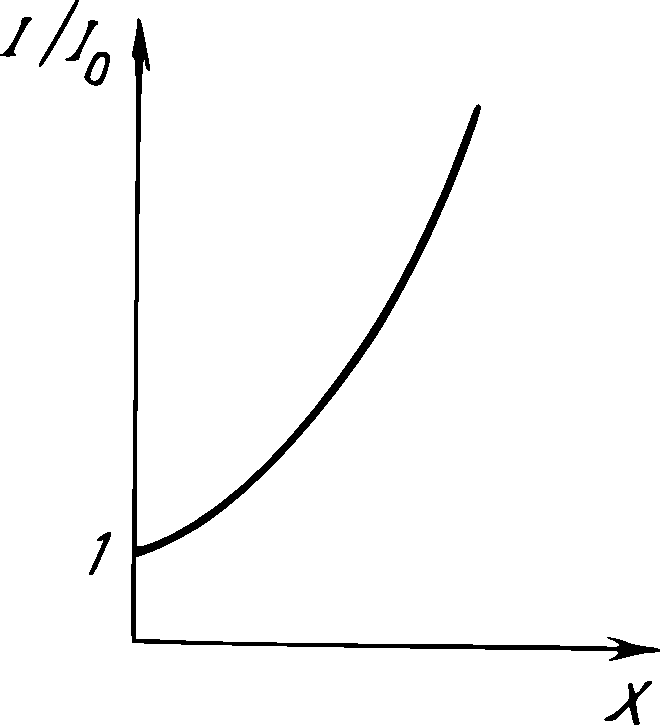
\includegraphics[width=0.7\textwidth]{figs/ch-39/fig-39-07.pdf}
\sidecaption{The intensity of light as a function of thickness of the medium.\zhcap{光强随介质厚度的变化。}\label{fig-39-07}}
\end{marginfigure}
where $\abs{\alpha} > 0$ is a positive quantity corresponding to the strengthening, rather than the weakening, of light passing through an active medium. At this the intensity of the light increases drastically with the thickness of the layer of the medium (\figr{fig-39-07}). In other words, the absorption factor $\alpha$ is a negative quantity for an active medium.
\zhpar{式中 $\abs{\alpha} > 0$ 为正值，它对应于穿过活性介质的光的增强而非减弱。这时光的强度随介质层厚度的增大而急剧增加（见\figr{fig-39-07}）。换言之，对于活性介质，吸收系数 $\alpha$ 为负值。}


\subsection{}\label{39.8.6} Three types of optical processes, illustrated in \figr{fig-39-08} can occur between two energy levels with the energies $E_{1}$ and $E_{2}$. Under conditions in which spontaneous emission can be neglected, i.e. radiation in which the excited atoms (or molecules or ions) spontaneously drop to the ground state, the optical properties of a medium are determined by competition between two processes: absorption and stimulated emission. 
\zhpar{两能级（能量分别为 $E_{1}$ 和 $E_{2}$）之间可能发生三种光学过程，如\figr{fig-39-08}所示。在可以忽略自发辐射（即受激原子、分子或离子自发跃迁到基态所产生的辐射）的条件下，介质的光学性质由两个过程之间的竞争决定：吸收和受激辐射。}



\begin{marginfigure}[-2cm] 
\centering
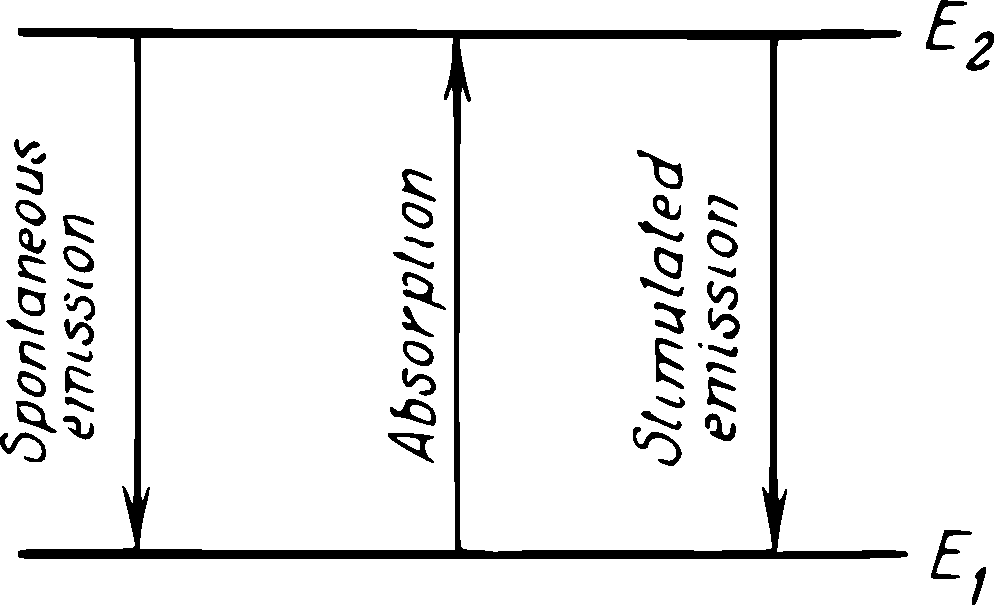
\includegraphics[width=\textwidth]{figs/ch-39/fig-39-08.pdf}
\sidecaption{The types of optical processes.\zhcap{光学过程的类型。}\label{fig-39-08}}
\end{marginfigure}


The number of events of absorption is proportional to the concentration $N_{1}$ of particles with the energy at the lower energy level. The number of events of stimulated emission is proportional to the concentration $N_{2}$ of particles at the upper energy level. The absorption factor a in the Bouguer-Lambert-Fabrikant law \ssect{39.8.5} is proportional to the difference between the numbers of events of absorption and stimulated emission. Thus 
\zhpar{吸收事件的数目与处于较低能级上的粒子浓度 $N_{1}$ 成正比，受激辐射事件的数目与处于较高能级上的粒子浓度 $N_{2}$ 成正比。布格-朗伯-法布里坎特定律 \ssect{39.8.5} 中的吸收系数 $\alpha$ 与吸收事件数和受激辐射事件数之差成正比。于是有：}
\begin{equation*}%
\alpha = k (N_{1} - N_{2}), 
\end{equation*}
where $k > 0$ is the proportionality factor.
\zhpar{式中 $k > 0$ 为比例系数。}

\subsection{}\label{39.8.7} When the system is in a state of thermodynamic equilibrium \ssect{8.3.3}, $N_{2} < N_{1}$ and $\alpha > 0$. This means that the number of events of absorption usually exceeds the number of transitions accompanied by stimulated emission of radiation. To obtain
a medium with a negative absorption factor it is necessary to
provide for a nonequilibrium state in the system, at which $N_{2}  > N_{1}$. Such states are said to be \redem{inverted}. In such a state the number of events of stimulated emission of radiation exceeds the number of events of absorption.
\zhpar{当系统处于热力学平衡状态 \ssect{8.3.3} 时，$N_{2} < N_{1}$，$\alpha > 0$。这意味着吸收事件的数目通常超过伴随受激辐射的跃迁数目。要获得吸收系数为负的介质，必须使系统处于非平衡状态，其中 $N_{2} > N_{1}$。这种状态称为粒子数\redem{反转}状态。在这种状态下，受激辐射事件的数目超过吸收事件的数目。}

\subsection{}\label{39.8.8} \redem{Lasers} (from the acronym for ``Light Amplification by the Stimulated Emission of Radiation''), or \redem{generators of coherent light}, are sources of light operating on the principle of stimulated emission of radiation in an active medium with an inverted population of energy levels \ssect{39.8.7}. If these devices operate in the optical range, they are known as \redem{lasers} proper. Those that operate in the range of ultrashort radiowaves are called \redem{masers} (Microwave Amplification by Stimulated Emission of Radiation).
\zhpar{\redem{激光器}（取自英文缩写 “Light Amplification by the Stimulated Emission of Radiation”，意为受激辐射光放大）或\redem{相干光发生器}，是基于活性介质中粒子数反转能级间受激辐射原理工作的光源 \ssect{39.8.7}。若这类器件工作于光学波段，则称为真正的\redem{激光器}。工作于超短无线电波段的器件称为\redem{微波激射器}（Microwave Amplification by Stimulated Emission of Radiation）。}

\subsection{}\label{39.8.9} The process of obtaining an inverted state (population inversion) in a medium \ssect{39.8.7}, required for laser operation, is called \redem{pumping the active medium}. In practice, pumping is accomplished by \redem{the three-level procedure}. One of the first lasers operating according to a three-level pumping procedure had a ruby for the active medium (alumina \ce{Al2O3} with the addition of chromium oxide \ce{Cr2O3}). In the crystal lattice of alumina, a part of the \ce{Al}
atoms are replaced by \ce{Cr^{3+}} ions, which serve as the active substance accomplishing the transitions with stimulated emission. 
\zhpar{获得介质中反转状态（粒子数反转）\ssect{39.8.7} 的过程是激光器工作所必需的，称为\redem{活性介质的泵浦}。在实际中，泵浦是通过\redem{三能级方法}实现的。最早按三能级泵浦方法工作的激光器之一，其活性介质为红宝石（掺有氧化铬 \ce{Cr2O3} 的氧化铝 \ce{Al2O3}）。在氧化铝晶格中，一部分 \ce{Al} 原子被 \ce{Cr^{3+}} 离子取代，这些离子作为活性物质完成受激辐射跃迁。}


\begin{marginfigure}%[-2cm] 
\centering
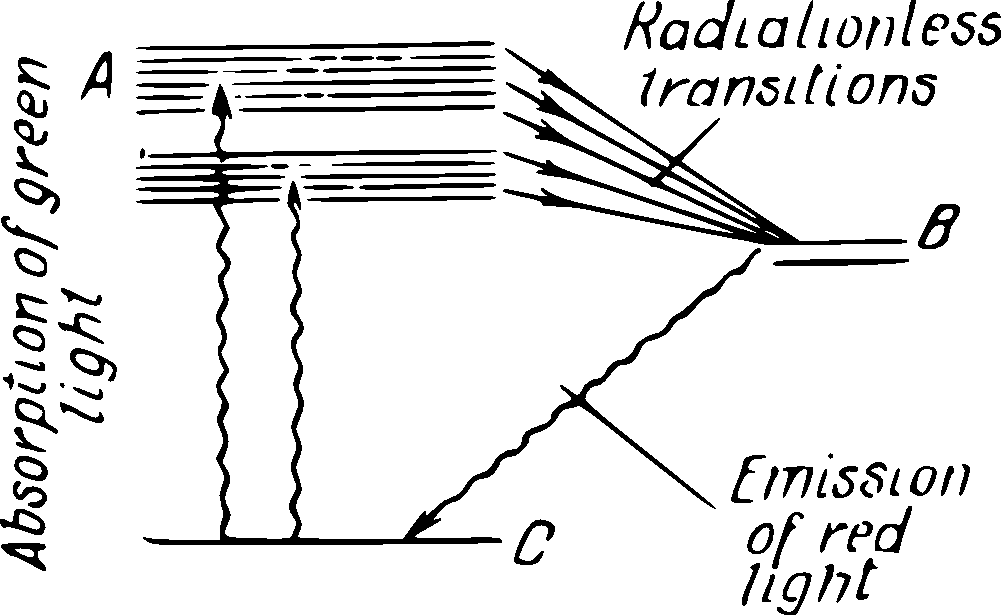
\includegraphics[width=\textwidth]{figs/ch-39/fig-39-09.pdf}
\sidecaption{A schematic diagram of three-level laser.\zhcap{三能级激光器的示意图。}\label{fig-39-09}}
\end{marginfigure}

A schematic diagram of the energy levels of \ce{Cr^{3+}} is given in \figr{fig-39-09}. The nearest to the ground-state level $C$ are two broad energy bands $A$ \ssect{41.8.2} and the double metastable level $B$. Intensive radiation, applied to the ruby by green light of a powerful pumping flashtube, filled with neon and krypton, transfers the chromium ions to the level of the $A$ band. From here radiationless  transitions occur to the $B$ level. The surplus energy is imparted to the ruby crystal lattice. As a result, a population inversion
of the chromium ions at the $B$ and $C$ levels is obtained \ssect{39.8.7} and the laser emits red light of the wavelengths \SI{6927}{\angstrom} and \SI{6943}{\angstrom},
corresponding to chromium ion transitions from level $B$ to level $C$.
\zhpar{\ce{Cr^{3+}} 的能级示意图见\figr{fig-39-09}。最接近基态能级 $C$ 的，是两个较宽的能带 $A$ \ssect{41.8.2} 和双重亚稳能级 $B$。由充有氖和氪的大功率脉冲闪光灯发出的强烈绿光照射红宝石，将铬离子激发到 $A$ 能带的能级上。从这里出发，发生无辐射跃迁到 $B$ 能级。多余的能量传给红宝石晶格。结果，$B$ 和 $C$ 能级上的铬离子获得粒子数反转 \ssect{39.8.7}，激光器发出波长为 \SI{6927}{\angstrom} 和 \SI{6943}{\angstrom} 的红光，它对应于铬离子从能级 $B$ 到能级 $C$ 的跃迁。}

\subsection{}\label{39.8.10} The avalanche-type increase in intensity in an active medium \ssect{39.8.5} indicates that such a medium operates as an semitransparent Mirror mirror
amplifier of electromagnetic waves. The light amplification effect in a laser is increased by passing the light many times through the same layer of the active medium. This takes place by means of the arrangement shown in \figr{fig-39-10}~(a). Photon $A$, travelling parallel to the axis of the active medium (a ruby rod) $\mathit{1}$, gives rise to an avalanche of photons moving in the same direction (\figr{fig-39-10}~(b)). 
\zhpar{活性介质中光强的雪崩式增长（参见 \ssect{39.8.5}）表明，这种介质起着电磁波放大器的作用，可视为半透明镜式的放大器。激光中光的放大效应，是通过让光多次通过同一层活性介质而增强的。这是借助\figr{fig-39-10}（a）所示的装置实现的。平行于活性介质（红宝石棒）$\mathit{1}$ 轴线运动的光子 $A$，引发了沿同一方向运动的光子雪崩（见\figr{fig-39-10}（b））。}


\begin{marginfigure}%[-2cm] 
\centering
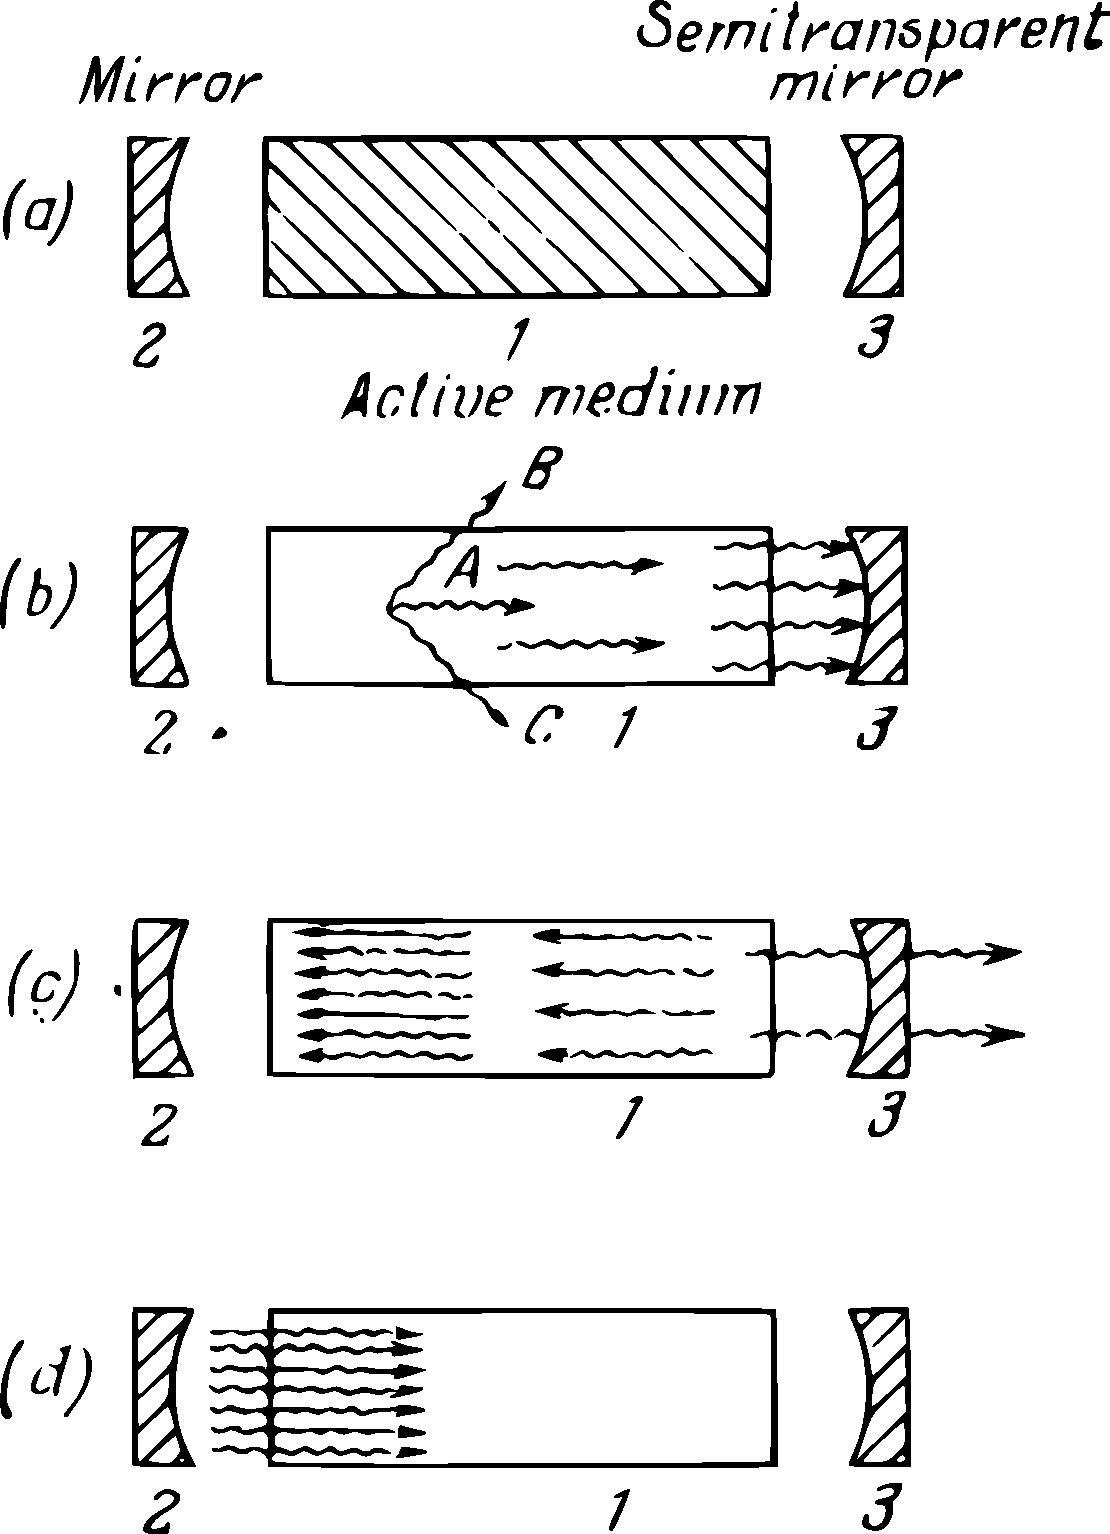
\includegraphics[width=\textwidth]{figs/ch-39/fig-39-10.pdf}
\sidecaption{The intensity of light as a function of thickness of the medium.\zhcap{光强随介质厚度的变化。}\label{fig-39-10}}
\end{marginfigure}

A part of this avalanche passes through semitransparent mirror $\mathit{3}$ and leaves the laser, and a part is reflected and increases again in the active medium (\figr{fig-39-10}~(c)). A part of the avalanche of photons that reaches the nontransparent mirror $\mathit{2}$ is absorbed by it but after reflection from this mirror the rest move in the same direction as the initial ``starting'' photon $A$
(\figr{fig-39-10}~(d)). The multiply amplified stream of photons, leaving the laser through the semitransparent mirror $\mathit{3}$, produces an extremely intense pencil of light rays, highly directional and with very little angular spread.
\zhpar{这一雪崩的一部分穿过半透明反射镜 $\mathit{3}$ 离开激光器，另一部分被反射后在活性介质中再次增强（见\figr{fig-39-10}（c））。到达不透明反射镜 $\mathit{2}$ 的部分光子雪崩被其吸收，但经该反射镜反射后，其余光子沿与最初的“起始”光子 $A$ 相同的方向运动（见\figr{fig-39-10}（d））。多次放大的光子流穿过半透明反射镜 $\mathit{3}$ 离开激光器，形成一束极强的光线，方向性极好，角发散极小。}

Photons $B$ and $C$ (\figr{fig-39-10}~(b)), travelling at an angle to the axis of the active medium, build up an avalanche of photons which, after multiple reflection, disappears from the medium and does not participate in light amplification. The high coherency, sharp directional properties and great intensity of laser radiation are the basis for its ever increasing application in science and engineering.
\zhpar{光子 $B$ 和 $C$（见\figr{fig-39-10}（b））与活性介质的轴线成一定角度运动，它们引发的光子雪崩经多次反射后离开介质，不参与光的放大。激光辐射的高度相干性、尖锐的方向性和很大的强度，是其在科学和工程技术中日益广泛应用的基础。}
% Local Variables:
% TeX-master: "handbook-physics"
% coding: utf-8
% End:
